\section{寄存器描述}
\regover{
{\hyperref[glb-gpio-cfg0]{gpio\_cfg0}}&
\\
\hline
{\hyperref[glb-gpio-cfg1]{gpio\_cfg1}}&
\\
\hline
{\hyperref[glb-gpio-cfg2]{gpio\_cfg2}}&
\\
\hline
{\hyperref[glb-gpio-cfg3]{gpio\_cfg3}}&
\\
\hline
{\hyperref[glb-gpio-cfg4]{gpio\_cfg4}}&
\\
\hline
{\hyperref[glb-gpio-cfg5]{gpio\_cfg5}}&
\\
\hline
{\hyperref[glb-gpio-cfg6]{gpio\_cfg6}}&
\\
\hline
{\hyperref[glb-gpio-cfg7]{gpio\_cfg7}}&
\\
\hline
{\hyperref[glb-gpio-cfg8]{gpio\_cfg8}}&
\\
\hline
{\hyperref[glb-gpio-cfg9]{gpio\_cfg9}}&
\\
\hline
{\hyperref[glb-gpio-cfg10]{gpio\_cfg10}}&
\\
\hline
{\hyperref[glb-gpio-cfg11]{gpio\_cfg11}}&
\\
\hline
{\hyperref[glb-gpio-cfg12]{gpio\_cfg12}}&
\\
\hline
{\hyperref[glb-gpio-cfg13]{gpio\_cfg13}}&
\\
\hline
{\hyperref[glb-gpio-cfg14]{gpio\_cfg14}}&
\\
\hline
{\hyperref[glb-gpio-cfg15]{gpio\_cfg15}}&
\\
\hline
{\hyperref[glb-gpio-cfg16]{gpio\_cfg16}}&
\\
\hline
{\hyperref[glb-gpio-cfg17]{gpio\_cfg17}}&
\\
\hline
{\hyperref[glb-gpio-cfg18]{gpio\_cfg18}}&
\\
\hline
{\hyperref[glb-gpio-cfg19]{gpio\_cfg19}}&
\\
\hline
{\hyperref[glb-gpio-cfg20]{gpio\_cfg20}}&
\\
\hline
{\hyperref[glb-gpio-cfg21]{gpio\_cfg21}}&
\\
\hline
{\hyperref[glb-gpio-cfg22]{gpio\_cfg22}}&
\\
\hline
{\hyperref[glb-gpio-cfg23]{gpio\_cfg23}}&
\\
\hline
{\hyperref[glb-gpio-cfg24]{gpio\_cfg24}}&
\\
\hline
{\hyperref[glb-gpio-cfg25]{gpio\_cfg25}}&
\\
\hline
{\hyperref[glb-gpio-cfg26]{gpio\_cfg26}}&
\\
\hline
{\hyperref[glb-gpio-cfg27]{gpio\_cfg27}}&
\\
\hline
{\hyperref[glb-gpio-cfg28]{gpio\_cfg28}}&
\\
\hline
{\hyperref[glb-gpio-cfg29]{gpio\_cfg29}}&
\\
\hline
{\hyperref[glb-gpio-cfg30]{gpio\_cfg30}}&
\\
\hline
{\hyperref[glb-gpio-cfg31]{gpio\_cfg31}}&
\\
\hline
{\hyperref[glb-gpio-cfg32]{gpio\_cfg32}}&
\\
\hline
{\hyperref[glb-gpio-cfg33]{gpio\_cfg33}}&
\\
\hline
{\hyperref[glb-gpio-cfg34]{gpio\_cfg34}}&
\\
\hline
{\hyperref[glb-gpio-cfg128]{gpio\_cfg128}}&
\\
\hline
{\hyperref[glb-gpio-cfg129]{gpio\_cfg129}}&
\\
\hline
{\hyperref[glb-gpio-cfg136]{gpio\_cfg136}}&
\\
\hline
{\hyperref[glb-gpio-cfg137]{gpio\_cfg137}}&
\\
\hline
{\hyperref[glb-gpio-cfg138]{gpio\_cfg138}}&
\\
\hline
{\hyperref[glb-gpio-cfg139]{gpio\_cfg139}}&
\\
\hline
{\hyperref[glb-gpio-cfg141]{gpio\_cfg141}}&
\\
\hline
{\hyperref[glb-gpio-cfg142]{gpio\_cfg142}}&
\\
\hline
{\hyperref[glb-gpio-cfg143]{gpio\_cfg143}}&
\\
\hline
{\hyperref[glb-gpio-cfg144]{gpio\_cfg144}}&
\\
\hline
}

\subsection{gpio\_cfg0}
\label{glb-gpio-cfg0}
地址:0x200008c4
 \begin{figure}[H]
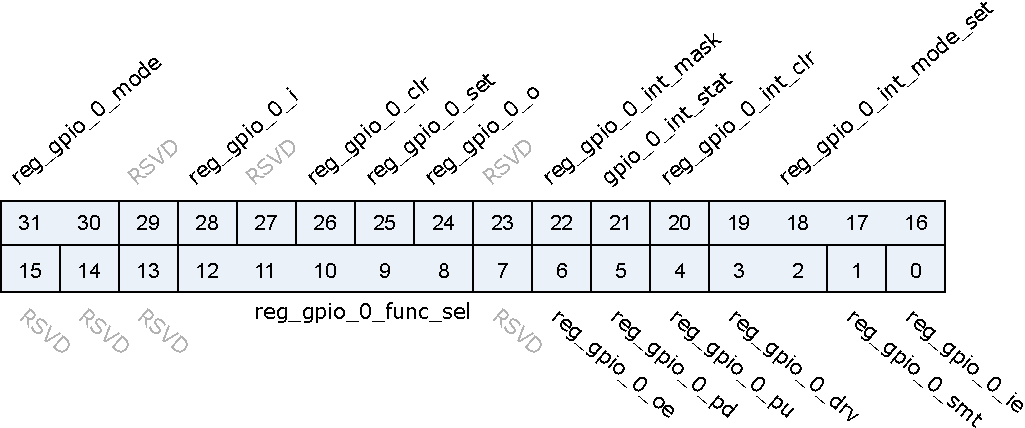
\includegraphics{glb_gpio_cfg0.pdf}
\end{figure}

\regdes{31:30&reg\_gpio\_0\_mode&r/w&0&When GPIO Function Selected to SWGPIO  \par 00 (Output Value Mode): GPIO Output by reg\_gpio\_x\_o Value  \par 01 (Set/Celar Mode     ) :GPIO Output set by reg\_gpio\_x\_set and clear by reg\_gpio\_x\_clr \par 10 : SWGPIO Source comes from  GPIO DMA (GPIO DMA Mode), GPIO Output value by gpio\_dma\_o \par 11: SWGPIO Source comes from  GPIO DMA (GPIO DMA Mode), GPIO Outout value by gpio\_dma\_set/gpio\_dma\_clr
\\\hline
29&RSVD& & & \\\hline
28&reg\_gpio\_0\_i&r&0&\\\hline
27&RSVD& & & \\\hline
26&reg\_gpio\_0\_clr&w1p&0&When SWGPIO @ Set/Clear Mode \par Set this bit will clear GPIO output value to 0,when set/clr at the same time, only set take effect
\\\hline
25&reg\_gpio\_0\_set&w1p&0&When SWGPIO @ Set/Clear Mode \par Set this bit will set GPIO output value to 1,when set/clr at the same time, only set take effect
\\\hline
24&reg\_gpio\_0\_o&r/w&0&When SWGPIO @ Output Value Mode \par 00 : GPIO Value changes according to this value \par 01 : GPIO Value Set by this register and clr by clr\_reg
\\\hline
23&RSVD& & & \\\hline
22&reg\_gpio\_0\_int\_mask&r/w&1&mask interrupt (1)\\\hline
21&gpio\_0\_int\_stat&r&0&interrupt status\\\hline
20&reg\_gpio\_0\_int\_clr&r/w&0&clear interrupt\\\hline
19:16&reg\_gpio\_0\_int\_mode\_set&r/w&0&0000 : sync falling edge trigger \par 0001 : sync rising edge trigger \par 0010 : sync low level trigger \par 0011 : sync high level trigger \par 01xx : sync rising \& falling edge trigger \par 1000 : async falling edge trigger \par 1001 : async rising edge trigger \par 1010 : async low level trigger \par 1011 : async high level trigger
\\\hline
15:13&RSVD& & & \\\hline
12:8&reg\_gpio\_0\_func\_sel&r/w&5'hB&GPIO Function Select (Default : SWGPIO)\\\hline
7&RSVD& & & \\\hline
6&reg\_gpio\_0\_oe&r/w&0&Register Controlled GPIO Output Enable (Used when GPIO Function select to Register Control GPIO)\\\hline
5&reg\_gpio\_0\_pd&r/w&0&GPIO Pull Down Control\\\hline
4&reg\_gpio\_0\_pu&r/w&0&GPIO Pull Up Control\\\hline
3:2&reg\_gpio\_0\_drv&r/w&0&GPIO Driving Control\\\hline
1&reg\_gpio\_0\_smt&r/w&1&GPIO SMT Control\\\hline
0&reg\_gpio\_0\_ie&r/w&0&GPIO Input Enable\\\hline

}
\subsection{gpio\_cfg1}
\label{glb-gpio-cfg1}
地址:0x200008c8
 \begin{figure}[H]
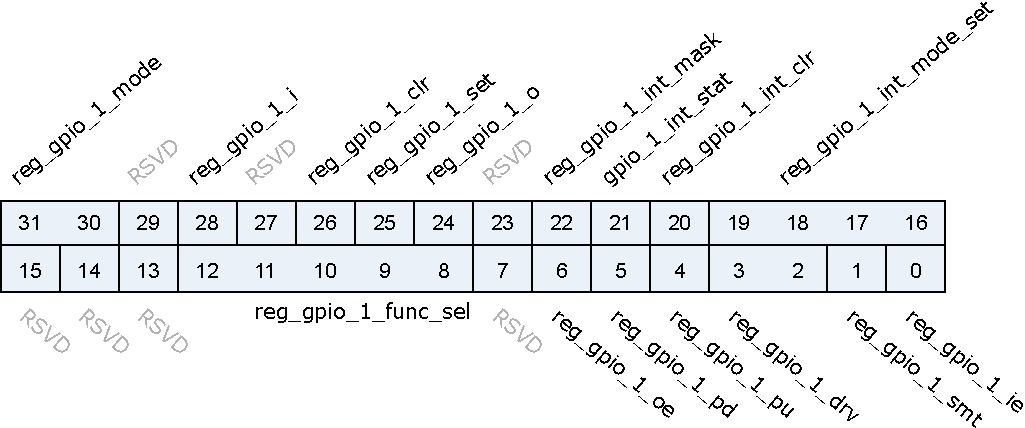
\includegraphics{glb_gpio_cfg1.pdf}
\end{figure}

\regdes{31:30&reg\_gpio\_1\_mode&r/w&0&When GPIO Function Selected to SWGPIO  \par 00 (Output Value Mode): GPIO Output by reg\_gpio\_x\_o Value  \par 01 (Set/Celar Mode     ) :GPIO Output set by reg\_gpio\_x\_set and clear by reg\_gpio\_x\_clr \par 10 : SWGPIO Source comes from  GPIO DMA (GPIO DMA Mode), GPIO Output value by gpio\_dma\_o \par 11: SWGPIO Source comes from  GPIO DMA (GPIO DMA Mode), GPIO Outout value by gpio\_dma\_set/gpio\_dma\_clr
\\\hline
29&RSVD& & & \\\hline
28&reg\_gpio\_1\_i&r&0&\\\hline
27&RSVD& & & \\\hline
26&reg\_gpio\_1\_clr&w1p&0&When SWGPIO @ Set/Clear Mode \par Set this bit will clear GPIO output value to 0,when set/clr at the same time, only set take effect
\\\hline
25&reg\_gpio\_1\_set&w1p&0&When SWGPIO @ Set/Clear Mode \par Set this bit will set GPIO output value to 1,when set/clr at the same time, only set take effect
\\\hline
24&reg\_gpio\_1\_o&r/w&0&When SWGPIO @ Output Value Mode \par 00 : GPIO Value changes according to this value \par 01 : GPIO Value Set by this register and clr by clr\_reg
\\\hline
23&RSVD& & & \\\hline
22&reg\_gpio\_1\_int\_mask&r/w&1&mask interrupt (1)\\\hline
21&gpio\_1\_int\_stat&r&0&interrupt status\\\hline
20&reg\_gpio\_1\_int\_clr&r/w&0&clear interrupt\\\hline
19:16&reg\_gpio\_1\_int\_mode\_set&r/w&0&0000 : sync falling edge trigger \par 0001 : sync rising edge trigger \par 0010 : sync low level trigger \par 0011 : sync high level trigger \par 01xx : sync rising \& falling edge trigger \par 1000 : async falling edge trigger \par 1001 : async rising edge trigger \par 1010 : async low level trigger \par 1011 : async high level trigger
\\\hline
15:13&RSVD& & & \\\hline
12:8&reg\_gpio\_1\_func\_sel&r/w&5'hB&GPIO Function Select (Default : SWGPIO)\\\hline
7&RSVD& & & \\\hline
6&reg\_gpio\_1\_oe&r/w&0&Register Controlled GPIO Output Enable (Used when GPIO Function select to Register Control GPIO)\\\hline
5&reg\_gpio\_1\_pd&r/w&0&GPIO Pull Down Control\\\hline
4&reg\_gpio\_1\_pu&r/w&0&GPIO Pull Up Control\\\hline
3:2&reg\_gpio\_1\_drv&r/w&0&GPIO Driving Control\\\hline
1&reg\_gpio\_1\_smt&r/w&1&GPIO SMT Control\\\hline
0&reg\_gpio\_1\_ie&r/w&0&GPIO Input Enable\\\hline

}
\subsection{gpio\_cfg2}
\label{glb-gpio-cfg2}
地址:0x200008cc
 \begin{figure}[H]
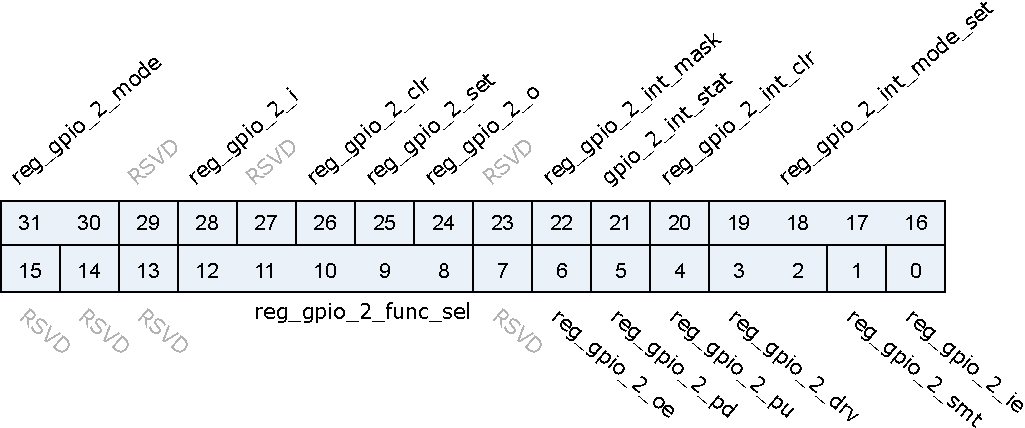
\includegraphics{glb_gpio_cfg2.pdf}
\end{figure}

\regdes{31:30&reg\_gpio\_2\_mode&r/w&0&When GPIO Function Selected to SWGPIO  \par 00 (Output Value Mode): GPIO Output by reg\_gpio\_x\_o Value  \par 01 (Set/Celar Mode     ) :GPIO Output set by reg\_gpio\_x\_set and clear by reg\_gpio\_x\_clr \par 10 : SWGPIO Source comes from  GPIO DMA (GPIO DMA Mode), GPIO Output value by gpio\_dma\_o \par 11: SWGPIO Source comes from  GPIO DMA (GPIO DMA Mode), GPIO Outout value by gpio\_dma\_set/gpio\_dma\_clr
\\\hline
29&RSVD& & & \\\hline
28&reg\_gpio\_2\_i&r&0&\\\hline
27&RSVD& & & \\\hline
26&reg\_gpio\_2\_clr&w1p&0&When SWGPIO @ Set/Clear Mode \par Set this bit will clear GPIO output value to 0,when set/clr at the same time, only set take effect
\\\hline
25&reg\_gpio\_2\_set&w1p&0&When SWGPIO @ Set/Clear Mode \par Set this bit will set GPIO output value to 1,when set/clr at the same time, only set take effect
\\\hline
24&reg\_gpio\_2\_o&r/w&0&When SWGPIO @ Output Value Mode \par 00 : GPIO Value changes according to this value \par 01 : GPIO Value Set by this register and clr by clr\_reg
\\\hline
23&RSVD& & & \\\hline
22&reg\_gpio\_2\_int\_mask&r/w&1&mask interrupt (1)\\\hline
21&gpio\_2\_int\_stat&r&0&interrupt status\\\hline
20&reg\_gpio\_2\_int\_clr&r/w&0&clear interrupt\\\hline
19:16&reg\_gpio\_2\_int\_mode\_set&r/w&0&0000 : sync falling edge trigger \par 0001 : sync rising edge trigger \par 0010 : sync low level trigger \par 0011 : sync high level trigger \par 01xx : sync rising \& falling edge trigger \par 1000 : async falling edge trigger \par 1001 : async rising edge trigger \par 1010 : async low level trigger \par 1011 : async high level trigger
\\\hline
15:13&RSVD& & & \\\hline
12:8&reg\_gpio\_2\_func\_sel&r/w&5'hB&GPIO Function Select (Default : SWGPIO)\\\hline
7&RSVD& & & \\\hline
6&reg\_gpio\_2\_oe&r/w&0&Register Controlled GPIO Output Enable (Used when GPIO Function select to Register Control GPIO)\\\hline
5&reg\_gpio\_2\_pd&r/w&0&GPIO Pull Down Control\\\hline
4&reg\_gpio\_2\_pu&r/w&0&GPIO Pull Up Control\\\hline
3:2&reg\_gpio\_2\_drv&r/w&0&GPIO Driving Control\\\hline
1&reg\_gpio\_2\_smt&r/w&1&GPIO SMT Control\\\hline
0&reg\_gpio\_2\_ie&r/w&0&GPIO Input Enable\\\hline

}
\subsection{gpio\_cfg3}
\label{glb-gpio-cfg3}
地址:0x200008d0
 \begin{figure}[H]
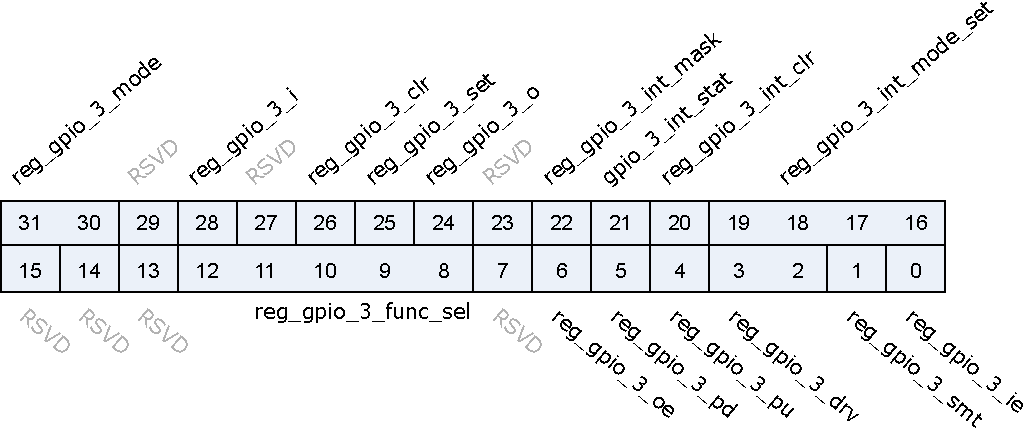
\includegraphics{glb_gpio_cfg3.pdf}
\end{figure}

\regdes{31:30&reg\_gpio\_3\_mode&r/w&0&When GPIO Function Selected to SWGPIO  \par 00 (Output Value Mode): GPIO Output by reg\_gpio\_x\_o Value  \par 01 (Set/Celar Mode     ) :GPIO Output set by reg\_gpio\_x\_set and clear by reg\_gpio\_x\_clr \par 10 : SWGPIO Source comes from  GPIO DMA (GPIO DMA Mode), GPIO Output value by gpio\_dma\_o \par 11: SWGPIO Source comes from  GPIO DMA (GPIO DMA Mode), GPIO Outout value by gpio\_dma\_set/gpio\_dma\_clr
\\\hline
29&RSVD& & & \\\hline
28&reg\_gpio\_3\_i&r&0&\\\hline
27&RSVD& & & \\\hline
26&reg\_gpio\_3\_clr&w1p&0&When SWGPIO @ Set/Clear Mode \par Set this bit will clear GPIO output value to 0,when set/clr at the same time, only set take effect
\\\hline
25&reg\_gpio\_3\_set&w1p&0&When SWGPIO @ Set/Clear Mode \par Set this bit will set GPIO output value to 1,when set/clr at the same time, only set take effect
\\\hline
24&reg\_gpio\_3\_o&r/w&0&When SWGPIO @ Output Value Mode \par 00 : GPIO Value changes according to this value \par 01 : GPIO Value Set by this register and clr by clr\_reg
\\\hline
23&RSVD& & & \\\hline
22&reg\_gpio\_3\_int\_mask&r/w&1&mask interrupt (1)\\\hline
21&gpio\_3\_int\_stat&r&0&interrupt status\\\hline
20&reg\_gpio\_3\_int\_clr&r/w&0&clear interrupt\\\hline
19:16&reg\_gpio\_3\_int\_mode\_set&r/w&0&0000 : sync falling edge trigger \par 0001 : sync rising edge trigger \par 0010 : sync low level trigger \par 0011 : sync high level trigger \par 01xx : sync rising \& falling edge trigger \par 1000 : async falling edge trigger \par 1001 : async rising edge trigger \par 1010 : async low level trigger \par 1011 : async high level trigger
\\\hline
15:13&RSVD& & & \\\hline
12:8&reg\_gpio\_3\_func\_sel&r/w&5'hB&GPIO Function Select (Default : SWGPIO)\\\hline
7&RSVD& & & \\\hline
6&reg\_gpio\_3\_oe&r/w&0&Register Controlled GPIO Output Enable (Used when GPIO Function select to Register Control GPIO)\\\hline
5&reg\_gpio\_3\_pd&r/w&0&GPIO Pull Down Control\\\hline
4&reg\_gpio\_3\_pu&r/w&0&GPIO Pull Up Control\\\hline
3:2&reg\_gpio\_3\_drv&r/w&0&GPIO Driving Control\\\hline
1&reg\_gpio\_3\_smt&r/w&1&GPIO SMT Control\\\hline
0&reg\_gpio\_3\_ie&r/w&0&GPIO Input Enable\\\hline

}
\subsection{gpio\_cfg4}
\label{glb-gpio-cfg4}
地址:0x200008d4
 \begin{figure}[H]
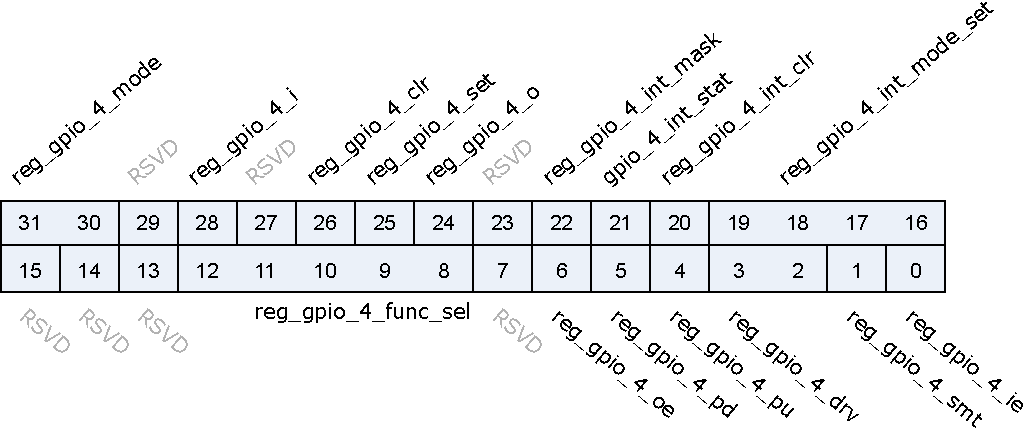
\includegraphics{glb_gpio_cfg4.pdf}
\end{figure}

\regdes{31:30&reg\_gpio\_4\_mode&r/w&0&When GPIO Function Selected to SWGPIO  \par 00 (Output Value Mode): GPIO Output by reg\_gpio\_x\_o Value  \par 01 (Set/Celar Mode     ) :GPIO Output set by reg\_gpio\_x\_set and clear by reg\_gpio\_x\_clr \par 10 : SWGPIO Source comes from  GPIO DMA (GPIO DMA Mode), GPIO Output value by gpio\_dma\_o \par 11: SWGPIO Source comes from  GPIO DMA (GPIO DMA Mode), GPIO Outout value by gpio\_dma\_set/gpio\_dma\_clr
\\\hline
29&RSVD& & & \\\hline
28&reg\_gpio\_4\_i&r&0&\\\hline
27&RSVD& & & \\\hline
26&reg\_gpio\_4\_clr&w1p&0&When SWGPIO @ Set/Clear Mode \par Set this bit will clear GPIO output value to 0,when set/clr at the same time, only set take effect
\\\hline
25&reg\_gpio\_4\_set&w1p&0&When SWGPIO @ Set/Clear Mode \par Set this bit will set GPIO output value to 1,when set/clr at the same time, only set take effect
\\\hline
24&reg\_gpio\_4\_o&r/w&0&When SWGPIO @ Output Value Mode \par 00 : GPIO Value changes according to this value \par 01 : GPIO Value Set by this register and clr by clr\_reg
\\\hline
23&RSVD& & & \\\hline
22&reg\_gpio\_4\_int\_mask&r/w&1&mask interrupt (1)\\\hline
21&gpio\_4\_int\_stat&r&0&interrupt status\\\hline
20&reg\_gpio\_4\_int\_clr&r/w&0&clear interrupt\\\hline
19:16&reg\_gpio\_4\_int\_mode\_set&r/w&0&0000 : sync falling edge trigger \par 0001 : sync rising edge trigger \par 0010 : sync low level trigger \par 0011 : sync high level trigger \par 01xx : sync rising \& falling edge trigger \par 1000 : async falling edge trigger \par 1001 : async rising edge trigger \par 1010 : async low level trigger \par 1011 : async high level trigger
\\\hline
15:13&RSVD& & & \\\hline
12:8&reg\_gpio\_4\_func\_sel&r/w&5'hB&GPIO Function Select (Default : SWGPIO)\\\hline
7&RSVD& & & \\\hline
6&reg\_gpio\_4\_oe&r/w&0&Register Controlled GPIO Output Enable (Used when GPIO Function select to Register Control GPIO)\\\hline
5&reg\_gpio\_4\_pd&r/w&0&GPIO Pull Down Control\\\hline
4&reg\_gpio\_4\_pu&r/w&0&GPIO Pull Up Control\\\hline
3:2&reg\_gpio\_4\_drv&r/w&0&GPIO Driving Control\\\hline
1&reg\_gpio\_4\_smt&r/w&1&GPIO SMT Control\\\hline
0&reg\_gpio\_4\_ie&r/w&0&GPIO Input Enable\\\hline

}
\subsection{gpio\_cfg5}
\label{glb-gpio-cfg5}
地址:0x200008d8
 \begin{figure}[H]
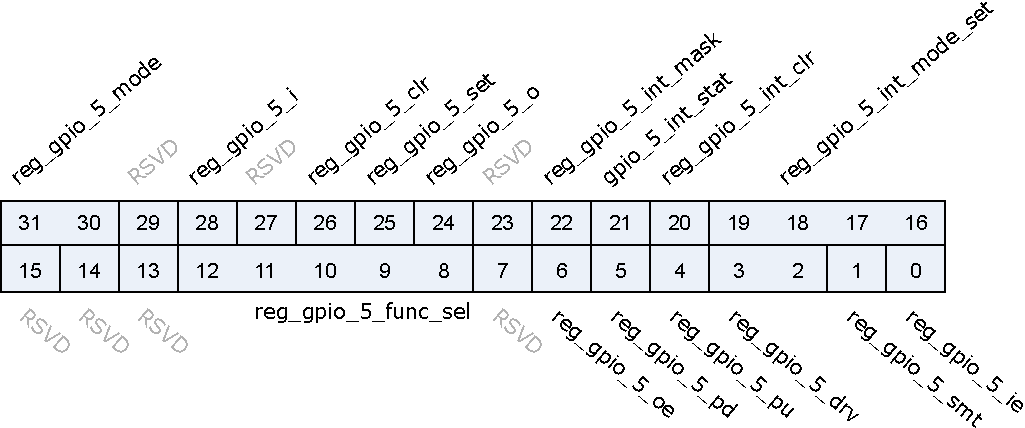
\includegraphics{glb_gpio_cfg5.pdf}
\end{figure}

\regdes{31:30&reg\_gpio\_5\_mode&r/w&0&When GPIO Function Selected to SWGPIO  \par 00 (Output Value Mode): GPIO Output by reg\_gpio\_x\_o Value  \par 01 (Set/Celar Mode     ) :GPIO Output set by reg\_gpio\_x\_set and clear by reg\_gpio\_x\_clr \par 10 : SWGPIO Source comes from  GPIO DMA (GPIO DMA Mode), GPIO Output value by gpio\_dma\_o \par 11: SWGPIO Source comes from  GPIO DMA (GPIO DMA Mode), GPIO Outout value by gpio\_dma\_set/gpio\_dma\_clr
\\\hline
29&RSVD& & & \\\hline
28&reg\_gpio\_5\_i&r&0&\\\hline
27&RSVD& & & \\\hline
26&reg\_gpio\_5\_clr&w1p&0&When SWGPIO @ Set/Clear Mode \par Set this bit will clear GPIO output value to 0,when set/clr at the same time, only set take effect
\\\hline
25&reg\_gpio\_5\_set&w1p&0&When SWGPIO @ Set/Clear Mode \par Set this bit will set GPIO output value to 1,when set/clr at the same time, only set take effect
\\\hline
24&reg\_gpio\_5\_o&r/w&0&When SWGPIO @ Output Value Mode \par 00 : GPIO Value changes according to this value \par 01 : GPIO Value Set by this register and clr by clr\_reg
\\\hline
23&RSVD& & & \\\hline
22&reg\_gpio\_5\_int\_mask&r/w&1&mask interrupt (1)\\\hline
21&gpio\_5\_int\_stat&r&0&interrupt status\\\hline
20&reg\_gpio\_5\_int\_clr&r/w&0&clear interrupt\\\hline
19:16&reg\_gpio\_5\_int\_mode\_set&r/w&0&0000 : sync falling edge trigger \par 0001 : sync rising edge trigger \par 0010 : sync low level trigger \par 0011 : sync high level trigger \par 01xx : sync rising \& falling edge trigger \par 1000 : async falling edge trigger \par 1001 : async rising edge trigger \par 1010 : async low level trigger \par 1011 : async high level trigger
\\\hline
15:13&RSVD& & & \\\hline
12:8&reg\_gpio\_5\_func\_sel&r/w&5'hB&GPIO Function Select (Default : SWGPIO)\\\hline
7&RSVD& & & \\\hline
6&reg\_gpio\_5\_oe&r/w&0&Register Controlled GPIO Output Enable (Used when GPIO Function select to Register Control GPIO)\\\hline
5&reg\_gpio\_5\_pd&r/w&0&GPIO Pull Down Control\\\hline
4&reg\_gpio\_5\_pu&r/w&0&GPIO Pull Up Control\\\hline
3:2&reg\_gpio\_5\_drv&r/w&0&GPIO Driving Control\\\hline
1&reg\_gpio\_5\_smt&r/w&1&GPIO SMT Control\\\hline
0&reg\_gpio\_5\_ie&r/w&0&GPIO Input Enable\\\hline

}
\subsection{gpio\_cfg6}
\label{glb-gpio-cfg6}
地址:0x200008dc
 \begin{figure}[H]
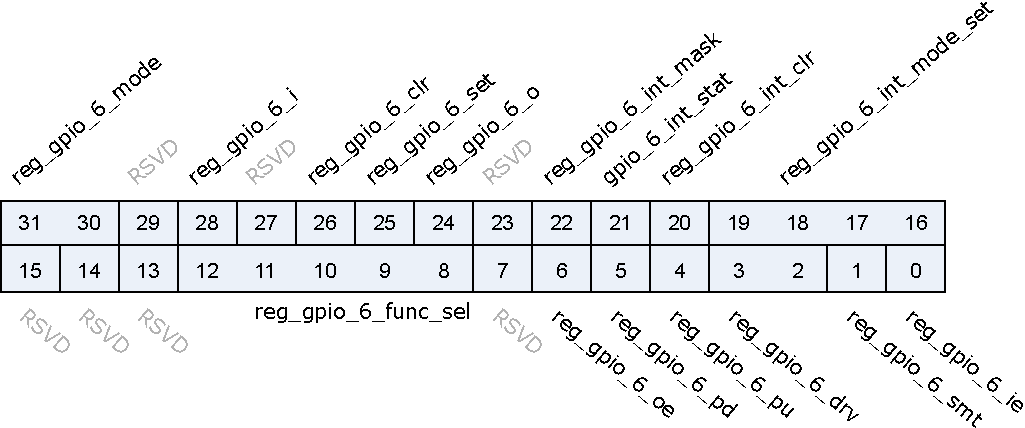
\includegraphics{glb_gpio_cfg6.pdf}
\end{figure}

\regdes{31:30&reg\_gpio\_6\_mode&r/w&0&When GPIO Function Selected to SWGPIO  \par 00 (Output Value Mode): GPIO Output by reg\_gpio\_x\_o Value  \par 01 (Set/Celar Mode     ) :GPIO Output set by reg\_gpio\_x\_set and clear by reg\_gpio\_x\_clr \par 10 : SWGPIO Source comes from  GPIO DMA (GPIO DMA Mode), GPIO Output value by gpio\_dma\_o \par 11: SWGPIO Source comes from  GPIO DMA (GPIO DMA Mode), GPIO Outout value by gpio\_dma\_set/gpio\_dma\_clr
\\\hline
29&RSVD& & & \\\hline
28&reg\_gpio\_6\_i&r&0&\\\hline
27&RSVD& & & \\\hline
26&reg\_gpio\_6\_clr&w1p&0&When SWGPIO @ Set/Clear Mode \par Set this bit will clear GPIO output value to 0,when set/clr at the same time, only set take effect
\\\hline
25&reg\_gpio\_6\_set&w1p&0&When SWGPIO @ Set/Clear Mode \par Set this bit will set GPIO output value to 1,when set/clr at the same time, only set take effect
\\\hline
24&reg\_gpio\_6\_o&r/w&0&When SWGPIO @ Output Value Mode \par 00 : GPIO Value changes according to this value \par 01 : GPIO Value Set by this register and clr by clr\_reg
\\\hline
23&RSVD& & & \\\hline
22&reg\_gpio\_6\_int\_mask&r/w&1&mask interrupt (1)\\\hline
21&gpio\_6\_int\_stat&r&0&interrupt status\\\hline
20&reg\_gpio\_6\_int\_clr&r/w&0&clear interrupt\\\hline
19:16&reg\_gpio\_6\_int\_mode\_set&r/w&0&0000 : sync falling edge trigger \par 0001 : sync rising edge trigger \par 0010 : sync low level trigger \par 0011 : sync high level trigger \par 01xx : sync rising \& falling edge trigger \par 1000 : async falling edge trigger \par 1001 : async rising edge trigger \par 1010 : async low level trigger \par 1011 : async high level trigger
\\\hline
15:13&RSVD& & & \\\hline
12:8&reg\_gpio\_6\_func\_sel&r/w&5'hB&GPIO Function Select (Default : SW-GPIO)\\\hline
7&RSVD& & & \\\hline
6&reg\_gpio\_6\_oe&r/w&0&Register Controlled GPIO Output Enable (Used when GPIO Function select to Register Control GPIO)\\\hline
5&reg\_gpio\_6\_pd&r/w&0&GPIO Pull Down Control\\\hline
4&reg\_gpio\_6\_pu&r/w&0&GPIO Pull Up Control\\\hline
3:2&reg\_gpio\_6\_drv&r/w&0&GPIO Driving Control\\\hline
1&reg\_gpio\_6\_smt&r/w&1&GPIO SMT Control\\\hline
0&reg\_gpio\_6\_ie&r/w&0&GPIO Input Enable\\\hline

}
\subsection{gpio\_cfg7}
\label{glb-gpio-cfg7}
地址:0x200008e0
 \begin{figure}[H]
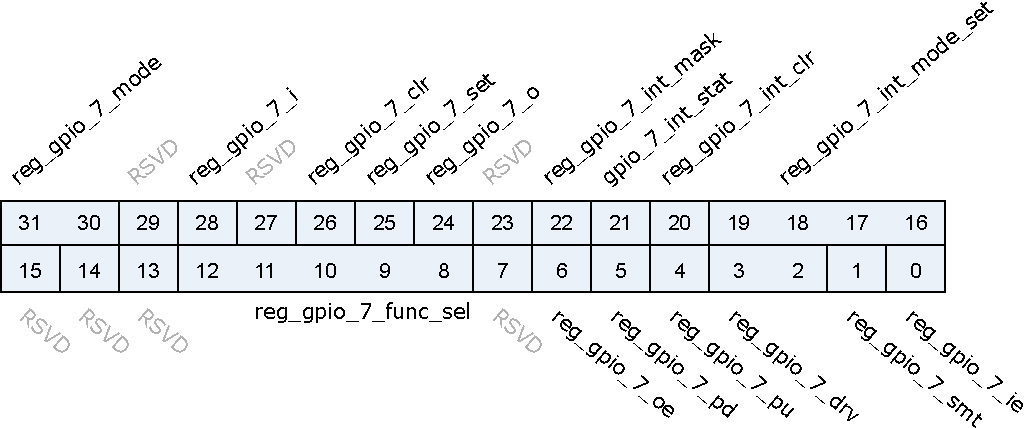
\includegraphics{glb_gpio_cfg7.pdf}
\end{figure}

\regdes{31:30&reg\_gpio\_7\_mode&r/w&0&When GPIO Function Selected to SWGPIO  \par 00 (Output Value Mode): GPIO Output by reg\_gpio\_x\_o Value  \par 01 (Set/Celar Mode     ) :GPIO Output set by reg\_gpio\_x\_set and clear by reg\_gpio\_x\_clr \par 10 : SWGPIO Source comes from  GPIO DMA (GPIO DMA Mode), GPIO Output value by gpio\_dma\_o \par 11: SWGPIO Source comes from  GPIO DMA (GPIO DMA Mode), GPIO Outout value by gpio\_dma\_set/gpio\_dma\_clr
\\\hline
29&RSVD& & & \\\hline
28&reg\_gpio\_7\_i&r&0&\\\hline
27&RSVD& & & \\\hline
26&reg\_gpio\_7\_clr&w1p&0&When SWGPIO @ Set/Clear Mode \par Set this bit will clear GPIO output value to 0,when set/clr at the same time, only set take effect
\\\hline
25&reg\_gpio\_7\_set&w1p&0&When SWGPIO @ Set/Clear Mode \par Set this bit will set GPIO output value to 1,when set/clr at the same time, only set take effect
\\\hline
24&reg\_gpio\_7\_o&r/w&0&When SWGPIO @ Output Value Mode \par 00 : GPIO Value changes according to this value \par 01 : GPIO Value Set by this register and clr by clr\_reg
\\\hline
23&RSVD& & & \\\hline
22&reg\_gpio\_7\_int\_mask&r/w&1&mask interrupt (1)\\\hline
21&gpio\_7\_int\_stat&r&0&interrupt status\\\hline
20&reg\_gpio\_7\_int\_clr&r/w&0&clear interrupt\\\hline
19:16&reg\_gpio\_7\_int\_mode\_set&r/w&0&0000 : sync falling edge trigger \par 0001 : sync rising edge trigger \par 0010 : sync low level trigger \par 0011 : sync high level trigger \par 01xx : sync rising \& falling edge trigger \par 1000 : async falling edge trigger \par 1001 : async rising edge trigger \par 1010 : async low level trigger \par 1011 : async high level trigger
\\\hline
15:13&RSVD& & & \\\hline
12:8&reg\_gpio\_7\_func\_sel&r/w&5'hB&GPIO Function Select (Default : SW-GPIO)\\\hline
7&RSVD& & & \\\hline
6&reg\_gpio\_7\_oe&r/w&0&Register Controlled GPIO Output Enable (Used when GPIO Function select to Register Control GPIO)\\\hline
5&reg\_gpio\_7\_pd&r/w&0&GPIO Pull Down Control\\\hline
4&reg\_gpio\_7\_pu&r/w&0&GPIO Pull Up Control\\\hline
3:2&reg\_gpio\_7\_drv&r/w&0&GPIO Driving Control\\\hline
1&reg\_gpio\_7\_smt&r/w&1&GPIO SMT Control\\\hline
0&reg\_gpio\_7\_ie&r/w&0&GPIO Input Enable\\\hline

}
\subsection{gpio\_cfg8}
\label{glb-gpio-cfg8}
地址:0x200008e4
 \begin{figure}[H]
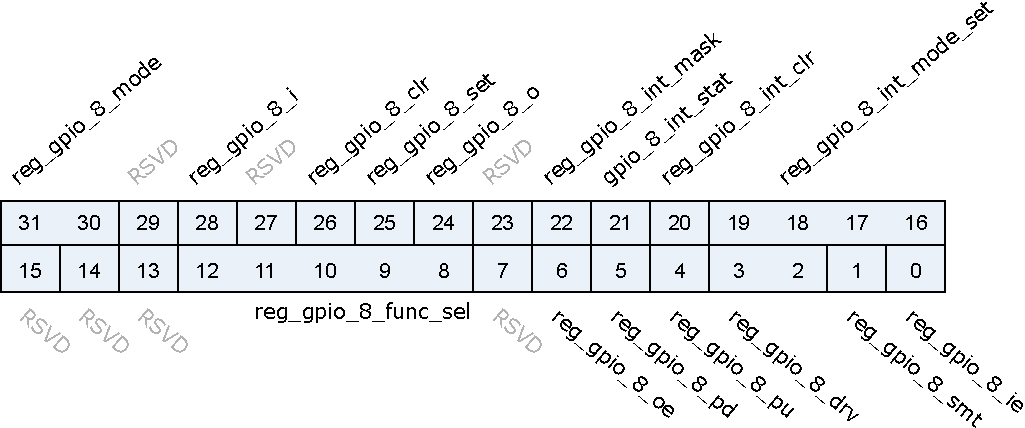
\includegraphics{glb_gpio_cfg8.pdf}
\end{figure}

\regdes{31:30&reg\_gpio\_8\_mode&r/w&0&When GPIO Function Selected to SWGPIO  \par 00 (Output Value Mode): GPIO Output by reg\_gpio\_x\_o Value  \par 01 (Set/Celar Mode     ) :GPIO Output set by reg\_gpio\_x\_set and clear by reg\_gpio\_x\_clr \par 10 : SWGPIO Source comes from  GPIO DMA (GPIO DMA Mode), GPIO Output value by gpio\_dma\_o \par 11: SWGPIO Source comes from  GPIO DMA (GPIO DMA Mode), GPIO Outout value by gpio\_dma\_set/gpio\_dma\_clr
\\\hline
29&RSVD& & & \\\hline
28&reg\_gpio\_8\_i&r&0&\\\hline
27&RSVD& & & \\\hline
26&reg\_gpio\_8\_clr&w1p&0&When SWGPIO @ Set/Clear Mode \par Set this bit will clear GPIO output value to 0,when set/clr at the same time, only set take effect
\\\hline
25&reg\_gpio\_8\_set&w1p&0&When SWGPIO @ Set/Clear Mode \par Set this bit will set GPIO output value to 1,when set/clr at the same time, only set take effect
\\\hline
24&reg\_gpio\_8\_o&r/w&0&When SWGPIO @ Output Value Mode \par 00 : GPIO Value changes according to this value \par 01 : GPIO Value Set by this register and clr by clr\_reg
\\\hline
23&RSVD& & & \\\hline
22&reg\_gpio\_8\_int\_mask&r/w&1&mask interrupt (1)\\\hline
21&gpio\_8\_int\_stat&r&0&interrupt status\\\hline
20&reg\_gpio\_8\_int\_clr&r/w&0&clear interrupt\\\hline
19:16&reg\_gpio\_8\_int\_mode\_set&r/w&0&0000 : sync falling edge trigger \par 0001 : sync rising edge trigger \par 0010 : sync low level trigger \par 0011 : sync high level trigger \par 01xx : sync rising \& falling edge trigger \par 1000 : async falling edge trigger \par 1001 : async rising edge trigger \par 1010 : async low level trigger \par 1011 : async high level trigger
\\\hline
15:13&RSVD& & & \\\hline
12:8&reg\_gpio\_8\_func\_sel&r/w&5'hB&GPIO Function Select (Default : SW-GPIO)\\\hline
7&RSVD& & & \\\hline
6&reg\_gpio\_8\_oe&r/w&0&Register Controlled GPIO Output Enable (Used when GPIO Function select to Register Control GPIO)\\\hline
5&reg\_gpio\_8\_pd&r/w&0&GPIO Pull Down Control\\\hline
4&reg\_gpio\_8\_pu&r/w&0&GPIO Pull Up Control\\\hline
3:2&reg\_gpio\_8\_drv&r/w&0&GPIO Driving Control\\\hline
1&reg\_gpio\_8\_smt&r/w&1&GPIO SMT Control\\\hline
0&reg\_gpio\_8\_ie&r/w&0&GPIO Input Enable\\\hline

}
\subsection{gpio\_cfg9}
\label{glb-gpio-cfg9}
地址:0x200008e8
 \begin{figure}[H]
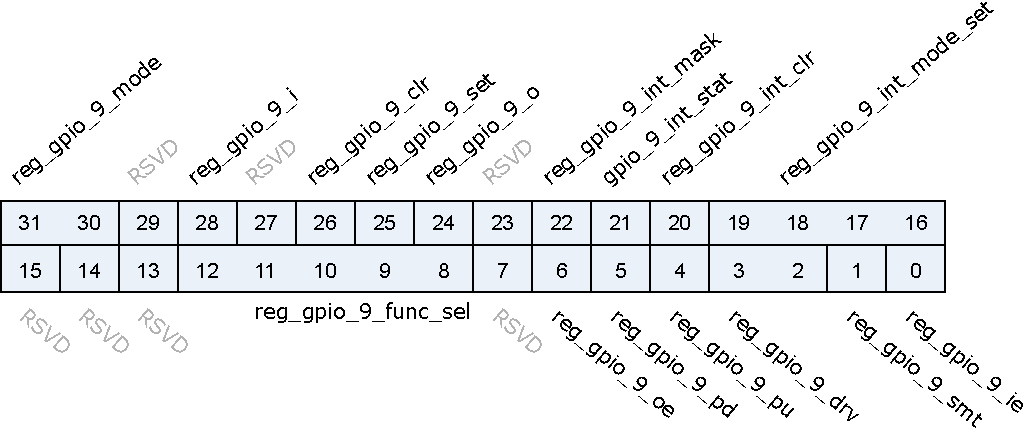
\includegraphics{glb_gpio_cfg9.pdf}
\end{figure}

\regdes{31:30&reg\_gpio\_9\_mode&r/w&0&When GPIO Function Selected to SWGPIO  \par 00 (Output Value Mode): GPIO Output by reg\_gpio\_x\_o Value  \par 01 (Set/Celar Mode     ) :GPIO Output set by reg\_gpio\_x\_set and clear by reg\_gpio\_x\_clr \par 10 : SWGPIO Source comes from  GPIO DMA (GPIO DMA Mode), GPIO Output value by gpio\_dma\_o \par 11: SWGPIO Source comes from  GPIO DMA (GPIO DMA Mode), GPIO Outout value by gpio\_dma\_set/gpio\_dma\_clr
\\\hline
29&RSVD& & & \\\hline
28&reg\_gpio\_9\_i&r&0&\\\hline
27&RSVD& & & \\\hline
26&reg\_gpio\_9\_clr&w1p&0&When SWGPIO @ Set/Clear Mode \par Set this bit will clear GPIO output value to 0,when set/clr at the same time, only set take effect
\\\hline
25&reg\_gpio\_9\_set&w1p&0&When SWGPIO @ Set/Clear Mode \par Set this bit will set GPIO output value to 1,when set/clr at the same time, only set take effect
\\\hline
24&reg\_gpio\_9\_o&r/w&0&When SWGPIO @ Output Value Mode \par 00 : GPIO Value changes according to this value \par 01 : GPIO Value Set by this register and clr by clr\_reg
\\\hline
23&RSVD& & & \\\hline
22&reg\_gpio\_9\_int\_mask&r/w&1&mask interrupt (1)\\\hline
21&gpio\_9\_int\_stat&r&0&interrupt status\\\hline
20&reg\_gpio\_9\_int\_clr&r/w&0&clear interrupt\\\hline
19:16&reg\_gpio\_9\_int\_mode\_set&r/w&0&0000 : sync falling edge trigger \par 0001 : sync rising edge trigger \par 0010 : sync low level trigger \par 0011 : sync high level trigger \par 01xx : sync rising \& falling edge trigger \par 1000 : async falling edge trigger \par 1001 : async rising edge trigger \par 1010 : async low level trigger \par 1011 : async high level trigger
\\\hline
15:13&RSVD& & & \\\hline
12:8&reg\_gpio\_9\_func\_sel&r/w&5'hB&GPIO Function Select (Default : SW-GPIO)\\\hline
7&RSVD& & & \\\hline
6&reg\_gpio\_9\_oe&r/w&0&Register Controlled GPIO Output Enable (Used when GPIO Function select to Register Control GPIO)\\\hline
5&reg\_gpio\_9\_pd&r/w&0&GPIO Pull Down Control\\\hline
4&reg\_gpio\_9\_pu&r/w&0&GPIO Pull Up Control\\\hline
3:2&reg\_gpio\_9\_drv&r/w&0&GPIO Driving Control\\\hline
1&reg\_gpio\_9\_smt&r/w&1&GPIO SMT Control\\\hline
0&reg\_gpio\_9\_ie&r/w&0&GPIO Input Enable\\\hline

}
\subsection{gpio\_cfg10}
\label{glb-gpio-cfg10}
地址:0x200008ec
 \begin{figure}[H]
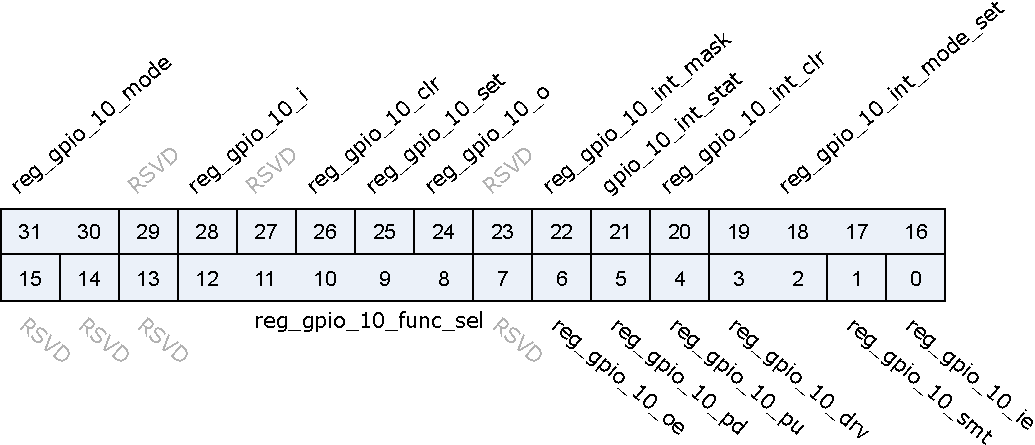
\includegraphics{glb_gpio_cfg10.pdf}
\end{figure}

\regdes{31:30&reg\_gpio\_10\_mode&r/w&0&When GPIO Function Selected to SWGPIO  \par 00 (Output Value Mode): GPIO Output by reg\_gpio\_x\_o Value  \par 01 (Set/Celar Mode     ) :GPIO Output set by reg\_gpio\_x\_set and clear by reg\_gpio\_x\_clr \par 10 : SWGPIO Source comes from  GPIO DMA (GPIO DMA Mode), GPIO Output value by gpio\_dma\_o \par 11: SWGPIO Source comes from  GPIO DMA (GPIO DMA Mode), GPIO Outout value by gpio\_dma\_set/gpio\_dma\_clr
\\\hline
29&RSVD& & & \\\hline
28&reg\_gpio\_10\_i&r&0&\\\hline
27&RSVD& & & \\\hline
26&reg\_gpio\_10\_clr&w1p&0&When SWGPIO @ Set/Clear Mode \par Set this bit will clear GPIO output value to 0,when set/clr at the same time, only set take effect
\\\hline
25&reg\_gpio\_10\_set&w1p&0&When SWGPIO @ Set/Clear Mode \par Set this bit will set GPIO output value to 1,when set/clr at the same time, only set take effect
\\\hline
24&reg\_gpio\_10\_o&r/w&0&When SWGPIO @ Output Value Mode \par 00 : GPIO Value changes according to this value \par 01 : GPIO Value Set by this register and clr by clr\_reg
\\\hline
23&RSVD& & & \\\hline
22&reg\_gpio\_10\_int\_mask&r/w&1&mask interrupt (1)\\\hline
21&gpio\_10\_int\_stat&r&0&interrupt status\\\hline
20&reg\_gpio\_10\_int\_clr&r/w&0&clear interrupt\\\hline
19:16&reg\_gpio\_10\_int\_mode\_set&r/w&0&0000 : sync falling edge trigger \par 0001 : sync rising edge trigger \par 0010 : sync low level trigger \par 0011 : sync high level trigger \par 01xx : sync rising \& falling edge trigger \par 1000 : async falling edge trigger \par 1001 : async rising edge trigger \par 1010 : async low level trigger \par 1011 : async high level trigger
\\\hline
15:13&RSVD& & & \\\hline
12:8&reg\_gpio\_10\_func\_sel&r/w&5'hF&GPIO Function Select (Default : CCI)\\\hline
7&RSVD& & & \\\hline
6&reg\_gpio\_10\_oe&r/w&0&Register Controlled GPIO Output Enable (Used when GPIO Function select to Register Control GPIO)\\\hline
5&reg\_gpio\_10\_pd&r/w&0&GPIO Pull Down Control\\\hline
4&reg\_gpio\_10\_pu&r/w&0&GPIO Pull Up Control\\\hline
3:2&reg\_gpio\_10\_drv&r/w&0&GPIO Driving Control\\\hline
1&reg\_gpio\_10\_smt&r/w&1&GPIO SMT Control\\\hline
0&reg\_gpio\_10\_ie&r/w&1&GPIO Input Enable\\\hline

}
\subsection{gpio\_cfg11}
\label{glb-gpio-cfg11}
地址:0x200008f0
 \begin{figure}[H]
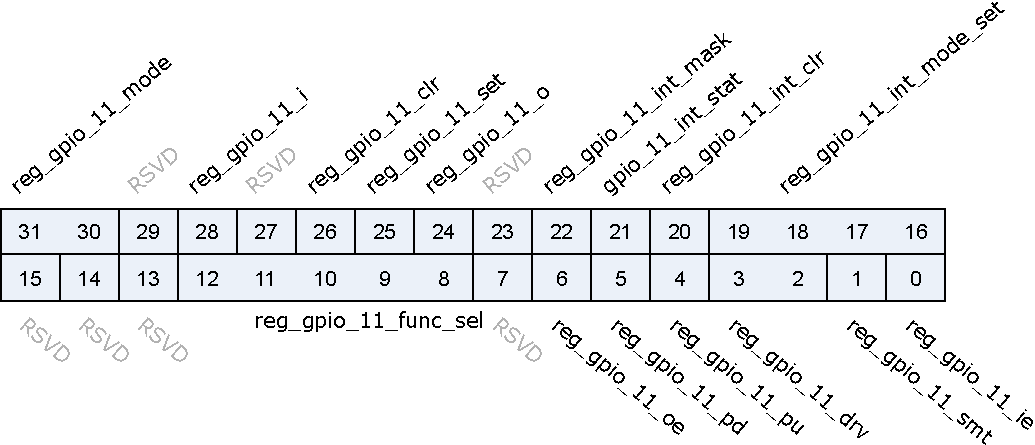
\includegraphics{glb_gpio_cfg11.pdf}
\end{figure}

\regdes{31:30&reg\_gpio\_11\_mode&r/w&0&When GPIO Function Selected to SWGPIO  \par 00 (Output Value Mode): GPIO Output by reg\_gpio\_x\_o Value  \par 01 (Set/Celar Mode     ) :GPIO Output set by reg\_gpio\_x\_set and clear by reg\_gpio\_x\_clr \par 10 : SWGPIO Source comes from  GPIO DMA (GPIO DMA Mode), GPIO Output value by gpio\_dma\_o \par 11: SWGPIO Source comes from  GPIO DMA (GPIO DMA Mode), GPIO Outout value by gpio\_dma\_set/gpio\_dma\_clr
\\\hline
29&RSVD& & & \\\hline
28&reg\_gpio\_11\_i&r&0&\\\hline
27&RSVD& & & \\\hline
26&reg\_gpio\_11\_clr&w1p&0&When SWGPIO @ Set/Clear Mode \par Set this bit will clear GPIO output value to 0,when set/clr at the same time, only set take effect
\\\hline
25&reg\_gpio\_11\_set&w1p&0&When SWGPIO @ Set/Clear Mode \par Set this bit will set GPIO output value to 1,when set/clr at the same time, only set take effect
\\\hline
24&reg\_gpio\_11\_o&r/w&0&When SWGPIO @ Output Value Mode \par 00 : GPIO Value changes according to this value \par 01 : GPIO Value Set by this register and clr by clr\_reg
\\\hline
23&RSVD& & & \\\hline
22&reg\_gpio\_11\_int\_mask&r/w&1&mask interrupt (1)\\\hline
21&gpio\_11\_int\_stat&r&0&interrupt status\\\hline
20&reg\_gpio\_11\_int\_clr&r/w&0&clear interrupt\\\hline
19:16&reg\_gpio\_11\_int\_mode\_set&r/w&0&0000 : sync falling edge trigger \par 0001 : sync rising edge trigger \par 0010 : sync low level trigger \par 0011 : sync high level trigger \par 01xx : sync rising \& falling edge trigger \par 1000 : async falling edge trigger \par 1001 : async rising edge trigger \par 1010 : async low level trigger \par 1011 : async high level trigger
\\\hline
15:13&RSVD& & & \\\hline
12:8&reg\_gpio\_11\_func\_sel&r/w&5'hF&GPIO Function Select (Default : CCI)\\\hline
7&RSVD& & & \\\hline
6&reg\_gpio\_11\_oe&r/w&0&Register Controlled GPIO Output Enable (Used when GPIO Function select to Register Control GPIO)\\\hline
5&reg\_gpio\_11\_pd&r/w&0&GPIO Pull Down Control\\\hline
4&reg\_gpio\_11\_pu&r/w&0&GPIO Pull Up Control\\\hline
3:2&reg\_gpio\_11\_drv&r/w&0&GPIO Driving Control\\\hline
1&reg\_gpio\_11\_smt&r/w&1&GPIO SMT Control\\\hline
0&reg\_gpio\_11\_ie&r/w&1&GPIO Input Enable\\\hline

}
\subsection{gpio\_cfg12}
\label{glb-gpio-cfg12}
地址:0x200008f4
 \begin{figure}[H]
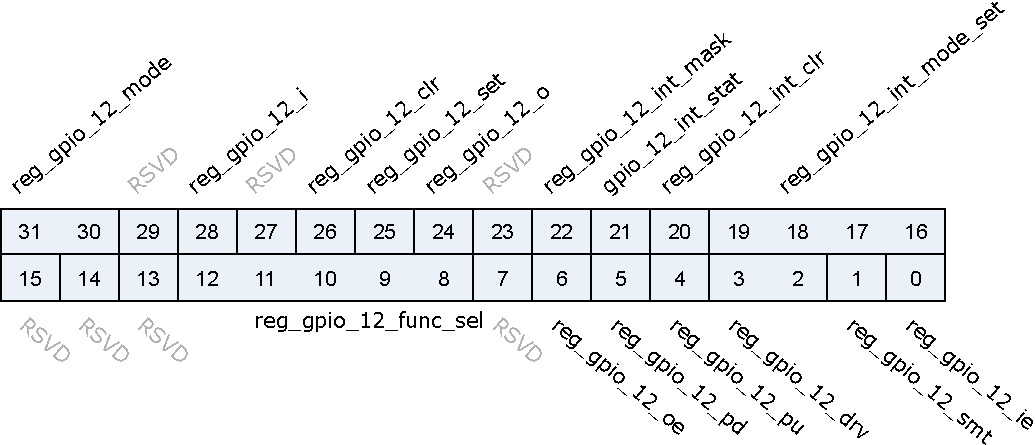
\includegraphics{glb_gpio_cfg12.pdf}
\end{figure}

\regdes{31:30&reg\_gpio\_12\_mode&r/w&0&When GPIO Function Selected to SWGPIO  \par 00 (Output Value Mode): GPIO Output by reg\_gpio\_x\_o Value  \par 01 (Set/Celar Mode     ) :GPIO Output set by reg\_gpio\_x\_set and clear by reg\_gpio\_x\_clr \par 10 : SWGPIO Source comes from  GPIO DMA (GPIO DMA Mode), GPIO Output value by gpio\_dma\_o \par 11: SWGPIO Source comes from  GPIO DMA (GPIO DMA Mode), GPIO Outout value by gpio\_dma\_set/gpio\_dma\_clr
\\\hline
29&RSVD& & & \\\hline
28&reg\_gpio\_12\_i&r&0&\\\hline
27&RSVD& & & \\\hline
26&reg\_gpio\_12\_clr&w1p&0&When SWGPIO @ Set/Clear Mode \par Set this bit will clear GPIO output value to 0,when set/clr at the same time, only set take effect
\\\hline
25&reg\_gpio\_12\_set&w1p&0&When SWGPIO @ Set/Clear Mode \par Set this bit will set GPIO output value to 1,when set/clr at the same time, only set take effect
\\\hline
24&reg\_gpio\_12\_o&r/w&0&When SWGPIO @ Output Value Mode \par 00 : GPIO Value changes according to this value \par 01 : GPIO Value Set by this register and clr by clr\_reg
\\\hline
23&RSVD& & & \\\hline
22&reg\_gpio\_12\_int\_mask&r/w&1&mask interrupt (1)\\\hline
21&gpio\_12\_int\_stat&r&0&interrupt status\\\hline
20&reg\_gpio\_12\_int\_clr&r/w&0&clear interrupt\\\hline
19:16&reg\_gpio\_12\_int\_mode\_set&r/w&0&0000 : sync falling edge trigger \par 0001 : sync rising edge trigger \par 0010 : sync low level trigger \par 0011 : sync high level trigger \par 01xx : sync rising \& falling edge trigger \par 1000 : async falling edge trigger \par 1001 : async rising edge trigger \par 1010 : async low level trigger \par 1011 : async high level trigger
\\\hline
15:13&RSVD& & & \\\hline
12:8&reg\_gpio\_12\_func\_sel&r/w&5'hF&GPIO Function Select (Default : CCI)\\\hline
7&RSVD& & & \\\hline
6&reg\_gpio\_12\_oe&r/w&0&Register Controlled GPIO Output Enable (Used when GPIO Function select to Register Control GPIO)\\\hline
5&reg\_gpio\_12\_pd&r/w&0&GPIO Pull Down Control\\\hline
4&reg\_gpio\_12\_pu&r/w&0&GPIO Pull Up Control\\\hline
3:2&reg\_gpio\_12\_drv&r/w&0&GPIO Driving Control\\\hline
1&reg\_gpio\_12\_smt&r/w&1&GPIO SMT Control\\\hline
0&reg\_gpio\_12\_ie&r/w&1&GPIO Input Enable\\\hline

}
\subsection{gpio\_cfg13}
\label{glb-gpio-cfg13}
地址:0x200008f8
 \begin{figure}[H]
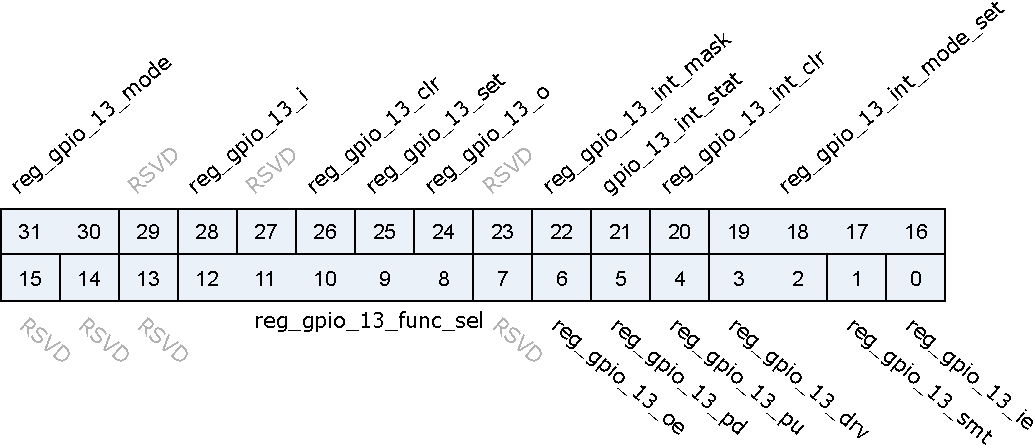
\includegraphics{glb_gpio_cfg13.pdf}
\end{figure}

\regdes{31:30&reg\_gpio\_13\_mode&r/w&0&When GPIO Function Selected to SWGPIO  \par 00 (Output Value Mode): GPIO Output by reg\_gpio\_x\_o Value  \par 01 (Set/Celar Mode     ) :GPIO Output set by reg\_gpio\_x\_set and clear by reg\_gpio\_x\_clr \par 10 : SWGPIO Source comes from  GPIO DMA (GPIO DMA Mode), GPIO Output value by gpio\_dma\_o \par 11: SWGPIO Source comes from  GPIO DMA (GPIO DMA Mode), GPIO Outout value by gpio\_dma\_set/gpio\_dma\_clr
\\\hline
29&RSVD& & & \\\hline
28&reg\_gpio\_13\_i&r&0&\\\hline
27&RSVD& & & \\\hline
26&reg\_gpio\_13\_clr&w1p&0&When SWGPIO @ Set/Clear Mode \par Set this bit will clear GPIO output value to 0,when set/clr at the same time, only set take effect
\\\hline
25&reg\_gpio\_13\_set&w1p&0&When SWGPIO @ Set/Clear Mode \par Set this bit will set GPIO output value to 1,when set/clr at the same time, only set take effect
\\\hline
24&reg\_gpio\_13\_o&r/w&0&When SWGPIO @ Output Value Mode \par 00 : GPIO Value changes according to this value \par 01 : GPIO Value Set by this register and clr by clr\_reg
\\\hline
23&RSVD& & & \\\hline
22&reg\_gpio\_13\_int\_mask&r/w&1&mask interrupt (1)\\\hline
21&gpio\_13\_int\_stat&r&0&interrupt status\\\hline
20&reg\_gpio\_13\_int\_clr&r/w&0&clear interrupt\\\hline
19:16&reg\_gpio\_13\_int\_mode\_set&r/w&0&0000 : sync falling edge trigger \par 0001 : sync rising edge trigger \par 0010 : sync low level trigger \par 0011 : sync high level trigger \par 01xx : sync rising \& falling edge trigger \par 1000 : async falling edge trigger \par 1001 : async rising edge trigger \par 1010 : async low level trigger \par 1011 : async high level trigger
\\\hline
15:13&RSVD& & & \\\hline
12:8&reg\_gpio\_13\_func\_sel&r/w&5'hB&GPIO Function Select (Default : SW-GPIO)\\\hline
7&RSVD& & & \\\hline
6&reg\_gpio\_13\_oe&r/w&0&Register Controlled GPIO Output Enable (Used when GPIO Function select to Register Control GPIO)\\\hline
5&reg\_gpio\_13\_pd&r/w&0&GPIO Pull Down Control\\\hline
4&reg\_gpio\_13\_pu&r/w&0&GPIO Pull Up Control\\\hline
3:2&reg\_gpio\_13\_drv&r/w&0&GPIO Driving Control\\\hline
1&reg\_gpio\_13\_smt&r/w&1&GPIO SMT Control\\\hline
0&reg\_gpio\_13\_ie&r/w&0&GPIO Input Enable\\\hline

}
\subsection{gpio\_cfg14}
\label{glb-gpio-cfg14}
地址:0x200008fc
 \begin{figure}[H]
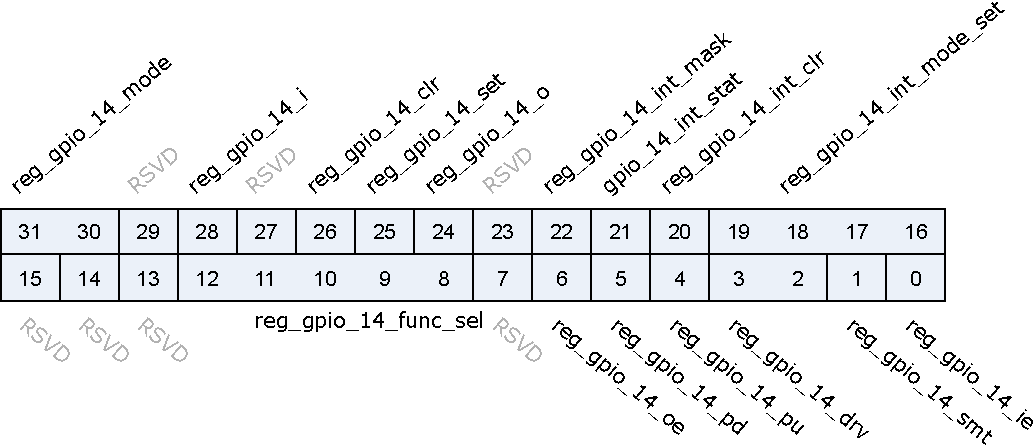
\includegraphics{glb_gpio_cfg14.pdf}
\end{figure}

\regdes{31:30&reg\_gpio\_14\_mode&r/w&0&When GPIO Function Selected to SWGPIO  \par 00 (Output Value Mode): GPIO Output by reg\_gpio\_x\_o Value  \par 01 (Set/Celar Mode     ) :GPIO Output set by reg\_gpio\_x\_set and clear by reg\_gpio\_x\_clr \par 10 : SWGPIO Source comes from  GPIO DMA (GPIO DMA Mode), GPIO Output value by gpio\_dma\_o \par 11: SWGPIO Source comes from  GPIO DMA (GPIO DMA Mode), GPIO Outout value by gpio\_dma\_set/gpio\_dma\_clr
\\\hline
29&RSVD& & & \\\hline
28&reg\_gpio\_14\_i&r&0&\\\hline
27&RSVD& & & \\\hline
26&reg\_gpio\_14\_clr&w1p&0&When SWGPIO @ Set/Clear Mode \par Set this bit will clear GPIO output value to 0,when set/clr at the same time, only set take effect
\\\hline
25&reg\_gpio\_14\_set&w1p&0&When SWGPIO @ Set/Clear Mode \par Set this bit will set GPIO output value to 1,when set/clr at the same time, only set take effect
\\\hline
24&reg\_gpio\_14\_o&r/w&0&When SWGPIO @ Output Value Mode \par 00 : GPIO Value changes according to this value \par 01 : GPIO Value Set by this register and clr by clr\_reg
\\\hline
23&RSVD& & & \\\hline
22&reg\_gpio\_14\_int\_mask&r/w&1&mask interrupt (1)\\\hline
21&gpio\_14\_int\_stat&r&0&interrupt status\\\hline
20&reg\_gpio\_14\_int\_clr&r/w&0&clear interrupt\\\hline
19:16&reg\_gpio\_14\_int\_mode\_set&r/w&0&0000 : sync falling edge trigger \par 0001 : sync rising edge trigger \par 0010 : sync low level trigger \par 0011 : sync high level trigger \par 01xx : sync rising \& falling edge trigger \par 1000 : async falling edge trigger \par 1001 : async rising edge trigger \par 1010 : async low level trigger \par 1011 : async high level trigger
\\\hline
15:13&RSVD& & & \\\hline
12:8&reg\_gpio\_14\_func\_sel&r/w&5'hB&GPIO Function Select (Default : SW-GPIO)\\\hline
7&RSVD& & & \\\hline
6&reg\_gpio\_14\_oe&r/w&0&Register Controlled GPIO Output Enable (Used when GPIO Function select to Register Control GPIO)\\\hline
5&reg\_gpio\_14\_pd&r/w&0&GPIO Pull Down Control\\\hline
4&reg\_gpio\_14\_pu&r/w&0&GPIO Pull Up Control\\\hline
3:2&reg\_gpio\_14\_drv&r/w&0&GPIO Driving Control\\\hline
1&reg\_gpio\_14\_smt&r/w&1&GPIO SMT Control\\\hline
0&reg\_gpio\_14\_ie&r/w&0&GPIO Input Enable\\\hline

}
\subsection{gpio\_cfg15}
\label{glb-gpio-cfg15}
地址:0x20000900
 \begin{figure}[H]
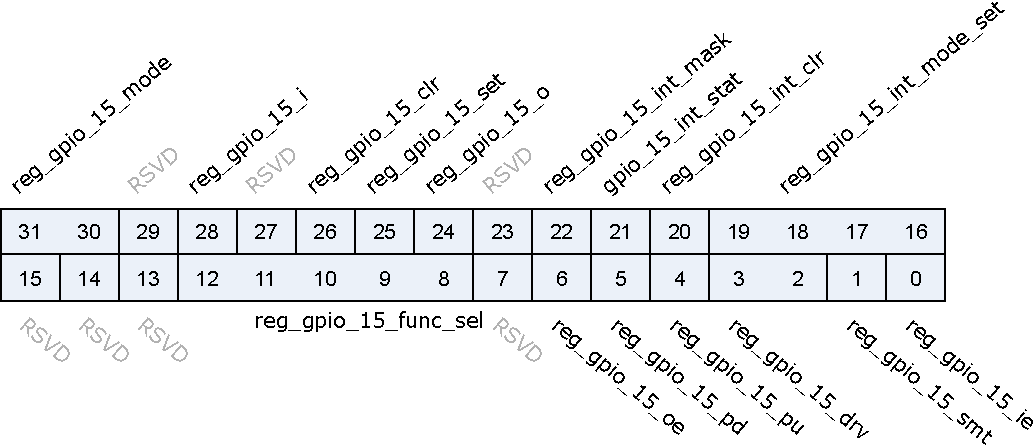
\includegraphics{glb_gpio_cfg15.pdf}
\end{figure}

\regdes{31:30&reg\_gpio\_15\_mode&r/w&0&When GPIO Function Selected to SWGPIO  \par 00 (Output Value Mode): GPIO Output by reg\_gpio\_x\_o Value  \par 01 (Set/Celar Mode     ) :GPIO Output set by reg\_gpio\_x\_set and clear by reg\_gpio\_x\_clr \par 10 : SWGPIO Source comes from  GPIO DMA (GPIO DMA Mode), GPIO Output value by gpio\_dma\_o \par 11: SWGPIO Source comes from  GPIO DMA (GPIO DMA Mode), GPIO Outout value by gpio\_dma\_set/gpio\_dma\_clr
\\\hline
29&RSVD& & & \\\hline
28&reg\_gpio\_15\_i&r&0&\\\hline
27&RSVD& & & \\\hline
26&reg\_gpio\_15\_clr&w1p&0&When SWGPIO @ Set/Clear Mode \par Set this bit will clear GPIO output value to 0,when set/clr at the same time, only set take effect
\\\hline
25&reg\_gpio\_15\_set&w1p&0&When SWGPIO @ Set/Clear Mode \par Set this bit will set GPIO output value to 1,when set/clr at the same time, only set take effect
\\\hline
24&reg\_gpio\_15\_o&r/w&0&When SWGPIO @ Output Value Mode \par 00 : GPIO Value changes according to this value \par 01 : GPIO Value Set by this register and clr by clr\_reg
\\\hline
23&RSVD& & & \\\hline
22&reg\_gpio\_15\_int\_mask&r/w&1&mask interrupt (1)\\\hline
21&gpio\_15\_int\_stat&r&0&interrupt status\\\hline
20&reg\_gpio\_15\_int\_clr&r/w&0&clear interrupt\\\hline
19:16&reg\_gpio\_15\_int\_mode\_set&r/w&0&0000 : sync falling edge trigger \par 0001 : sync rising edge trigger \par 0010 : sync low level trigger \par 0011 : sync high level trigger \par 01xx : sync rising \& falling edge trigger \par 1000 : async falling edge trigger \par 1001 : async rising edge trigger \par 1010 : async low level trigger \par 1011 : async high level trigger
\\\hline
15:13&RSVD& & & \\\hline
12:8&reg\_gpio\_15\_func\_sel&r/w&5'hB&GPIO Function Select (Default : SW-GPIO)\\\hline
7&RSVD& & & \\\hline
6&reg\_gpio\_15\_oe&r/w&0&Register Controlled GPIO Output Enable (Used when GPIO Function select to Register Control GPIO)\\\hline
5&reg\_gpio\_15\_pd&r/w&0&GPIO Pull Down Control\\\hline
4&reg\_gpio\_15\_pu&r/w&0&GPIO Pull Up Control\\\hline
3:2&reg\_gpio\_15\_drv&r/w&0&GPIO Driving Control\\\hline
1&reg\_gpio\_15\_smt&r/w&1&GPIO SMT Control\\\hline
0&reg\_gpio\_15\_ie&r/w&0&GPIO Input Enable\\\hline

}
\subsection{gpio\_cfg16}
\label{glb-gpio-cfg16}
地址:0x20000904
 \begin{figure}[H]
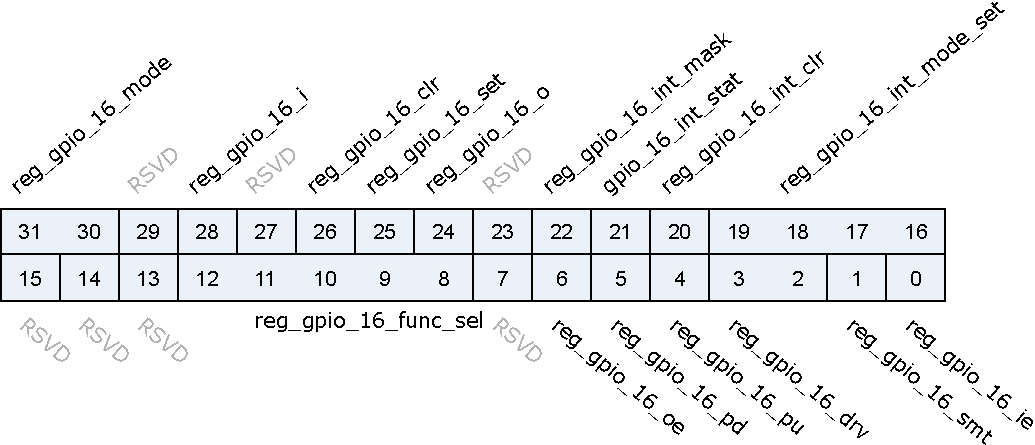
\includegraphics{glb_gpio_cfg16.pdf}
\end{figure}

\regdes{31:30&reg\_gpio\_16\_mode&r/w&0&When GPIO Function Selected to SWGPIO  \par 00 (Output Value Mode): GPIO Output by reg\_gpio\_x\_o Value  \par 01 (Set/Celar Mode     ) :GPIO Output set by reg\_gpio\_x\_set and clear by reg\_gpio\_x\_clr \par 10 : SWGPIO Source comes from  GPIO DMA (GPIO DMA Mode), GPIO Output value by gpio\_dma\_o \par 11: SWGPIO Source comes from  GPIO DMA (GPIO DMA Mode), GPIO Outout value by gpio\_dma\_set/gpio\_dma\_clr
\\\hline
29&RSVD& & & \\\hline
28&reg\_gpio\_16\_i&r&0&\\\hline
27&RSVD& & & \\\hline
26&reg\_gpio\_16\_clr&w1p&0&When SWGPIO @ Set/Clear Mode \par Set this bit will clear GPIO output value to 0,when set/clr at the same time, only set take effect
\\\hline
25&reg\_gpio\_16\_set&w1p&0&When SWGPIO @ Set/Clear Mode \par Set this bit will set GPIO output value to 1,when set/clr at the same time, only set take effect
\\\hline
24&reg\_gpio\_16\_o&r/w&0&When SWGPIO @ Output Value Mode \par 00 : GPIO Value changes according to this value \par 01 : GPIO Value Set by this register and clr by clr\_reg
\\\hline
23&RSVD& & & \\\hline
22&reg\_gpio\_16\_int\_mask&r/w&1&mask interrupt (1)\\\hline
21&gpio\_16\_int\_stat&r&0&interrupt status\\\hline
20&reg\_gpio\_16\_int\_clr&r/w&0&clear interrupt\\\hline
19:16&reg\_gpio\_16\_int\_mode\_set&r/w&0&0000 : sync falling edge trigger \par 0001 : sync rising edge trigger \par 0010 : sync low level trigger \par 0011 : sync high level trigger \par 01xx : sync rising \& falling edge trigger \par 1000 : async falling edge trigger \par 1001 : async rising edge trigger \par 1010 : async low level trigger \par 1011 : async high level trigger
\\\hline
15:13&RSVD& & & \\\hline
12:8&reg\_gpio\_16\_func\_sel&r/w&5'hB&GPIO Function Select (Default : SW-GPIO)\\\hline
7&RSVD& & & \\\hline
6&reg\_gpio\_16\_oe&r/w&0&Register Controlled GPIO Output Enable (Used when GPIO Function select to Register Control GPIO)\\\hline
5&reg\_gpio\_16\_pd&r/w&0&GPIO Pull Down Control\\\hline
4&reg\_gpio\_16\_pu&r/w&0&GPIO Pull Up Control\\\hline
3:2&reg\_gpio\_16\_drv&r/w&0&GPIO Driving Control\\\hline
1&reg\_gpio\_16\_smt&r/w&1&GPIO SMT Control\\\hline
0&reg\_gpio\_16\_ie&r/w&0&GPIO Input Enable\\\hline

}
\subsection{gpio\_cfg17}
\label{glb-gpio-cfg17}
地址:0x20000908
 \begin{figure}[H]
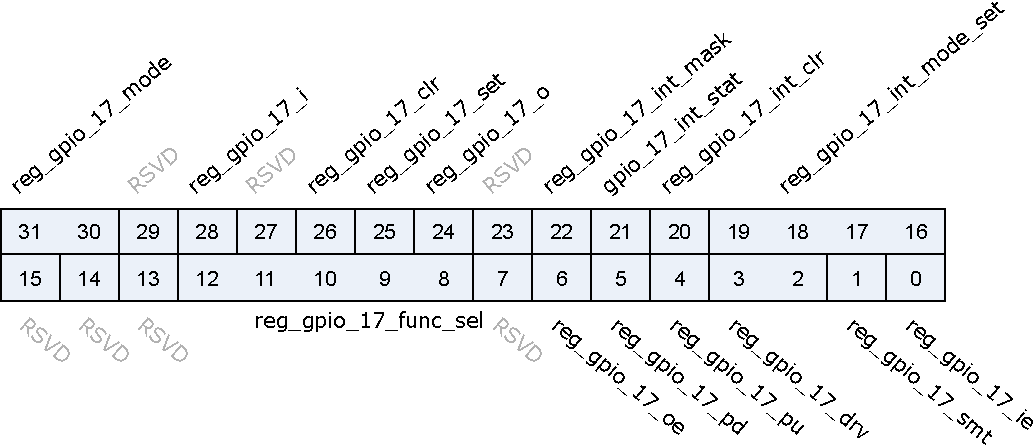
\includegraphics{glb_gpio_cfg17.pdf}
\end{figure}

\regdes{31:30&reg\_gpio\_17\_mode&r/w&0&When GPIO Function Selected to SWGPIO  \par 00 (Output Value Mode): GPIO Output by reg\_gpio\_x\_o Value  \par 01 (Set/Celar Mode     ) :GPIO Output set by reg\_gpio\_x\_set and clear by reg\_gpio\_x\_clr \par 10 : SWGPIO Source comes from  GPIO DMA (GPIO DMA Mode), GPIO Output value by gpio\_dma\_o \par 11: SWGPIO Source comes from  GPIO DMA (GPIO DMA Mode), GPIO Outout value by gpio\_dma\_set/gpio\_dma\_clr
\\\hline
29&RSVD& & & \\\hline
28&reg\_gpio\_17\_i&r&0&\\\hline
27&RSVD& & & \\\hline
26&reg\_gpio\_17\_clr&w1p&0&When SWGPIO @ Set/Clear Mode \par Set this bit will clear GPIO output value to 0,when set/clr at the same time, only set take effect
\\\hline
25&reg\_gpio\_17\_set&w1p&0&When SWGPIO @ Set/Clear Mode \par Set this bit will set GPIO output value to 1,when set/clr at the same time, only set take effect
\\\hline
24&reg\_gpio\_17\_o&r/w&0&When SWGPIO @ Output Value Mode \par 00 : GPIO Value changes according to this value \par 01 : GPIO Value Set by this register and clr by clr\_reg
\\\hline
23&RSVD& & & \\\hline
22&reg\_gpio\_17\_int\_mask&r/w&1&mask interrupt (1)\\\hline
21&gpio\_17\_int\_stat&r&0&interrupt status\\\hline
20&reg\_gpio\_17\_int\_clr&r/w&0&clear interrupt\\\hline
19:16&reg\_gpio\_17\_int\_mode\_set&r/w&0&0000 : sync falling edge trigger \par 0001 : sync rising edge trigger \par 0010 : sync low level trigger \par 0011 : sync high level trigger \par 01xx : sync rising \& falling edge trigger \par 1000 : async falling edge trigger \par 1001 : async rising edge trigger \par 1010 : async low level trigger \par 1011 : async high level trigger
\\\hline
15:13&RSVD& & & \\\hline
12:8&reg\_gpio\_17\_func\_sel&r/w&5'hB&GPIO Function Select (Default : SW-GPIO)\\\hline
7&RSVD& & & \\\hline
6&reg\_gpio\_17\_oe&r/w&0&Register Controlled GPIO Output Enable (Used when GPIO Function select to Register Control GPIO)\\\hline
5&reg\_gpio\_17\_pd&r/w&0&GPIO Pull Down Control\\\hline
4&reg\_gpio\_17\_pu&r/w&0&GPIO Pull Up Control\\\hline
3:2&reg\_gpio\_17\_drv&r/w&0&GPIO Driving Control\\\hline
1&reg\_gpio\_17\_smt&r/w&1&GPIO SMT Control\\\hline
0&reg\_gpio\_17\_ie&r/w&0&GPIO Input Enable\\\hline

}
\subsection{gpio\_cfg18}
\label{glb-gpio-cfg18}
地址:0x2000090c
 \begin{figure}[H]
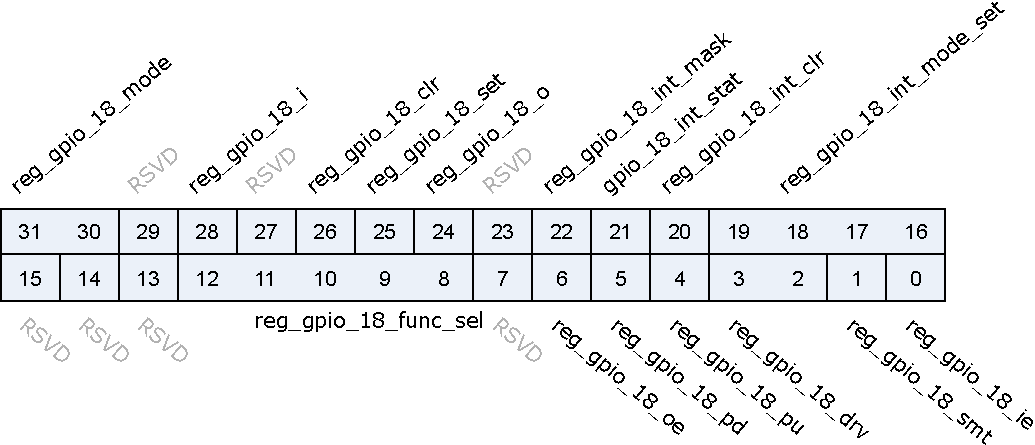
\includegraphics{glb_gpio_cfg18.pdf}
\end{figure}

\regdes{31:30&reg\_gpio\_18\_mode&r/w&0&When GPIO Function Selected to SWGPIO  \par 00 (Output Value Mode): GPIO Output by reg\_gpio\_x\_o Value  \par 01 (Set/Celar Mode     ) :GPIO Output set by reg\_gpio\_x\_set and clear by reg\_gpio\_x\_clr \par 10 : SWGPIO Source comes from  GPIO DMA (GPIO DMA Mode), GPIO Output value by gpio\_dma\_o \par 11: SWGPIO Source comes from  GPIO DMA (GPIO DMA Mode), GPIO Outout value by gpio\_dma\_set/gpio\_dma\_clr
\\\hline
29&RSVD& & & \\\hline
28&reg\_gpio\_18\_i&r&0&\\\hline
27&RSVD& & & \\\hline
26&reg\_gpio\_18\_clr&w1p&0&When SWGPIO @ Set/Clear Mode \par Set this bit will clear GPIO output value to 0,when set/clr at the same time, only set take effect
\\\hline
25&reg\_gpio\_18\_set&w1p&0&When SWGPIO @ Set/Clear Mode \par Set this bit will set GPIO output value to 1,when set/clr at the same time, only set take effect
\\\hline
24&reg\_gpio\_18\_o&r/w&0&When SWGPIO @ Output Value Mode \par 00 : GPIO Value changes according to this value \par 01 : GPIO Value Set by this register and clr by clr\_reg
\\\hline
23&RSVD& & & \\\hline
22&reg\_gpio\_18\_int\_mask&r/w&1&mask interrupt (1)\\\hline
21&gpio\_18\_int\_stat&r&0&interrupt status\\\hline
20&reg\_gpio\_18\_int\_clr&r/w&0&clear interrupt\\\hline
19:16&reg\_gpio\_18\_int\_mode\_set&r/w&0&0000 : sync falling edge trigger \par 0001 : sync rising edge trigger \par 0010 : sync low level trigger \par 0011 : sync high level trigger \par 01xx : sync rising \& falling edge trigger \par 1000 : async falling edge trigger \par 1001 : async rising edge trigger \par 1010 : async low level trigger \par 1011 : async high level trigger
\\\hline
15:13&RSVD& & & \\\hline
12:8&reg\_gpio\_18\_func\_sel&r/w&5'hB&GPIO Function Select (Default : SW-GPIO)\\\hline
7&RSVD& & & \\\hline
6&reg\_gpio\_18\_oe&r/w&0&Register Controlled GPIO Output Enable (Used when GPIO Function select to Register Control GPIO)\\\hline
5&reg\_gpio\_18\_pd&r/w&0&GPIO Pull Down Control\\\hline
4&reg\_gpio\_18\_pu&r/w&0&GPIO Pull Up Control\\\hline
3:2&reg\_gpio\_18\_drv&r/w&0&GPIO Driving Control\\\hline
1&reg\_gpio\_18\_smt&r/w&1&GPIO SMT Control\\\hline
0&reg\_gpio\_18\_ie&r/w&0&GPIO Input Enable\\\hline

}
\subsection{gpio\_cfg19}
\label{glb-gpio-cfg19}
地址:0x20000910
 \begin{figure}[H]
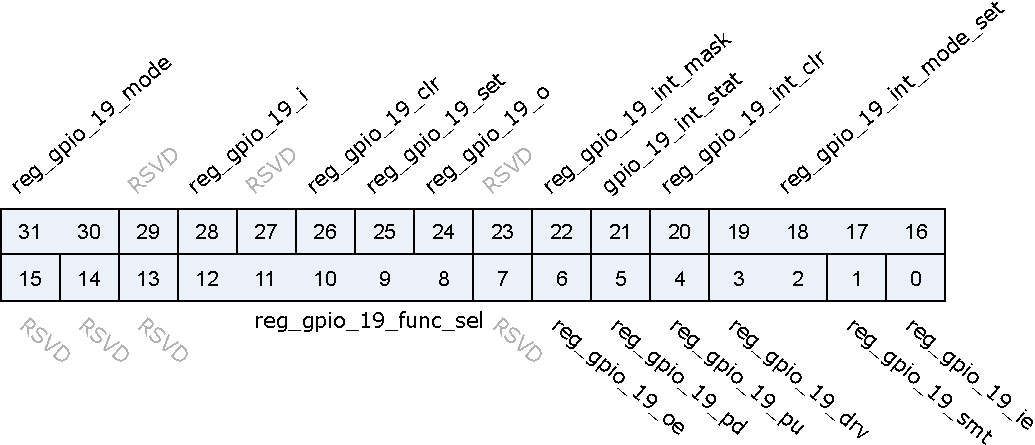
\includegraphics{glb_gpio_cfg19.pdf}
\end{figure}

\regdes{31:30&reg\_gpio\_19\_mode&r/w&0&When GPIO Function Selected to SWGPIO  \par 00 (Output Value Mode): GPIO Output by reg\_gpio\_x\_o Value  \par 01 (Set/Celar Mode     ) :GPIO Output set by reg\_gpio\_x\_set and clear by reg\_gpio\_x\_clr \par 10 : SWGPIO Source comes from  GPIO DMA (GPIO DMA Mode), GPIO Output value by gpio\_dma\_o \par 11: SWGPIO Source comes from  GPIO DMA (GPIO DMA Mode), GPIO Outout value by gpio\_dma\_set/gpio\_dma\_clr
\\\hline
29&RSVD& & & \\\hline
28&reg\_gpio\_19\_i&r&0&\\\hline
27&RSVD& & & \\\hline
26&reg\_gpio\_19\_clr&w1p&0&When SWGPIO @ Set/Clear Mode \par Set this bit will clear GPIO output value to 0,when set/clr at the same time, only set take effect
\\\hline
25&reg\_gpio\_19\_set&w1p&0&When SWGPIO @ Set/Clear Mode \par Set this bit will set GPIO output value to 1,when set/clr at the same time, only set take effect
\\\hline
24&reg\_gpio\_19\_o&r/w&0&When SWGPIO @ Output Value Mode \par 00 : GPIO Value changes according to this value \par 01 : GPIO Value Set by this register and clr by clr\_reg
\\\hline
23&RSVD& & & \\\hline
22&reg\_gpio\_19\_int\_mask&r/w&1&mask interrupt (1)\\\hline
21&gpio\_19\_int\_stat&r&0&interrupt status\\\hline
20&reg\_gpio\_19\_int\_clr&r/w&0&clear interrupt\\\hline
19:16&reg\_gpio\_19\_int\_mode\_set&r/w&0&0000 : sync falling edge trigger \par 0001 : sync rising edge trigger \par 0010 : sync low level trigger \par 0011 : sync high level trigger \par 01xx : sync rising \& falling edge trigger \par 1000 : async falling edge trigger \par 1001 : async rising edge trigger \par 1010 : async low level trigger \par 1011 : async high level trigger
\\\hline
15:13&RSVD& & & \\\hline
12:8&reg\_gpio\_19\_func\_sel&r/w&5'hB&GPIO Function Select (Default : SW-GPIO)\\\hline
7&RSVD& & & \\\hline
6&reg\_gpio\_19\_oe&r/w&0&Register Controlled GPIO Output Enable (Used when GPIO Function select to Register Control GPIO)\\\hline
5&reg\_gpio\_19\_pd&r/w&0&GPIO Pull Down Control\\\hline
4&reg\_gpio\_19\_pu&r/w&0&GPIO Pull Up Control\\\hline
3:2&reg\_gpio\_19\_drv&r/w&0&GPIO Driving Control\\\hline
1&reg\_gpio\_19\_smt&r/w&1&GPIO SMT Control\\\hline
0&reg\_gpio\_19\_ie&r/w&0&GPIO Input Enable\\\hline

}
\subsection{gpio\_cfg20}
\label{glb-gpio-cfg20}
地址:0x20000914
 \begin{figure}[H]
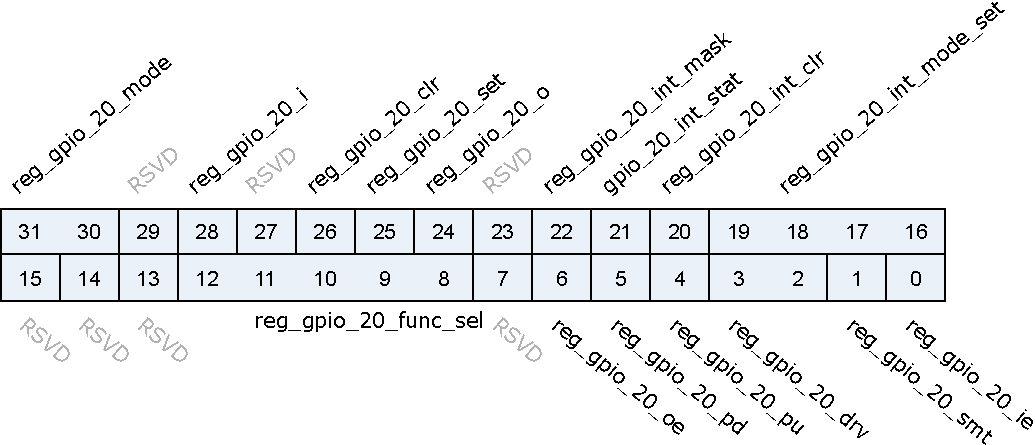
\includegraphics{glb_gpio_cfg20.pdf}
\end{figure}

\regdes{31:30&reg\_gpio\_20\_mode&r/w&0&When GPIO Function Selected to SWGPIO  \par 00 (Output Value Mode): GPIO Output by reg\_gpio\_x\_o Value  \par 01 (Set/Celar Mode     ) :GPIO Output set by reg\_gpio\_x\_set and clear by reg\_gpio\_x\_clr \par 10 : SWGPIO Source comes from  GPIO DMA (GPIO DMA Mode), GPIO Output value by gpio\_dma\_o \par 11: SWGPIO Source comes from  GPIO DMA (GPIO DMA Mode), GPIO Outout value by gpio\_dma\_set/gpio\_dma\_clr
\\\hline
29&RSVD& & & \\\hline
28&reg\_gpio\_20\_i&r&0&\\\hline
27&RSVD& & & \\\hline
26&reg\_gpio\_20\_clr&w1p&0&When SWGPIO @ Set/Clear Mode \par Set this bit will clear GPIO output value to 0,when set/clr at the same time, only set take effect
\\\hline
25&reg\_gpio\_20\_set&w1p&0&When SWGPIO @ Set/Clear Mode \par Set this bit will set GPIO output value to 1,when set/clr at the same time, only set take effect
\\\hline
24&reg\_gpio\_20\_o&r/w&0&When SWGPIO @ Output Value Mode \par 00 : GPIO Value changes according to this value \par 01 : GPIO Value Set by this register and clr by clr\_reg
\\\hline
23&RSVD& & & \\\hline
22&reg\_gpio\_20\_int\_mask&r/w&1&mask interrupt (1)\\\hline
21&gpio\_20\_int\_stat&r&0&interrupt status\\\hline
20&reg\_gpio\_20\_int\_clr&r/w&0&clear interrupt\\\hline
19:16&reg\_gpio\_20\_int\_mode\_set&r/w&0&0000 : sync falling edge trigger \par 0001 : sync rising edge trigger \par 0010 : sync low level trigger \par 0011 : sync high level trigger \par 01xx : sync rising \& falling edge trigger \par 1000 : async falling edge trigger \par 1001 : async rising edge trigger \par 1010 : async low level trigger \par 1011 : async high level trigger
\\\hline
15:13&RSVD& & & \\\hline
12:8&reg\_gpio\_20\_func\_sel&r/w&5'hB&GPIO Function Select (Default : SW-GPIO)\\\hline
7&RSVD& & & \\\hline
6&reg\_gpio\_20\_oe&r/w&0&Register Controlled GPIO Output Enable (Used when GPIO Function select to Register Control GPIO)\\\hline
5&reg\_gpio\_20\_pd&r/w&0&GPIO Pull Down Control\\\hline
4&reg\_gpio\_20\_pu&r/w&0&GPIO Pull Up Control\\\hline
3:2&reg\_gpio\_20\_drv&r/w&0&GPIO Driving Control\\\hline
1&reg\_gpio\_20\_smt&r/w&1&GPIO SMT Control\\\hline
0&reg\_gpio\_20\_ie&r/w&0&GPIO Input Enable\\\hline

}
\subsection{gpio\_cfg21}
\label{glb-gpio-cfg21}
地址:0x20000918
 \begin{figure}[H]
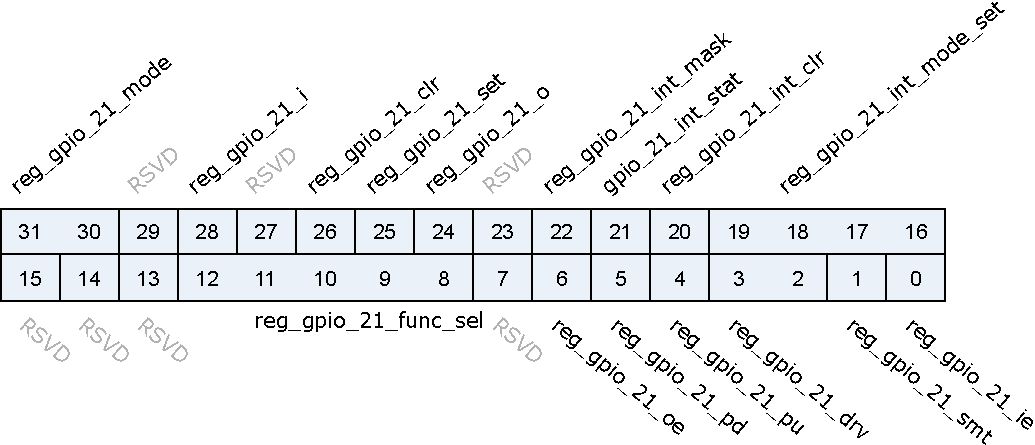
\includegraphics{glb_gpio_cfg21.pdf}
\end{figure}

\regdes{31:30&reg\_gpio\_21\_mode&r/w&0&When GPIO Function Selected to SWGPIO  \par 00 (Output Value Mode): GPIO Output by reg\_gpio\_x\_o Value  \par 01 (Set/Celar Mode     ) :GPIO Output set by reg\_gpio\_x\_set and clear by reg\_gpio\_x\_clr \par 10 : SWGPIO Source comes from  GPIO DMA (GPIO DMA Mode), GPIO Output value by gpio\_dma\_o \par 11: SWGPIO Source comes from  GPIO DMA (GPIO DMA Mode), GPIO Outout value by gpio\_dma\_set/gpio\_dma\_clr
\\\hline
29&RSVD& & & \\\hline
28&reg\_gpio\_21\_i&r&0&\\\hline
27&RSVD& & & \\\hline
26&reg\_gpio\_21\_clr&w1p&0&When SWGPIO @ Set/Clear Mode \par Set this bit will clear GPIO output value to 0,when set/clr at the same time, only set take effect
\\\hline
25&reg\_gpio\_21\_set&w1p&0&When SWGPIO @ Set/Clear Mode \par Set this bit will set GPIO output value to 1,when set/clr at the same time, only set take effect
\\\hline
24&reg\_gpio\_21\_o&r/w&0&When SWGPIO @ Output Value Mode \par 00 : GPIO Value changes according to this value \par 01 : GPIO Value Set by this register and clr by clr\_reg
\\\hline
23&RSVD& & & \\\hline
22&reg\_gpio\_21\_int\_mask&r/w&1&mask interrupt (1)\\\hline
21&gpio\_21\_int\_stat&r&0&interrupt status\\\hline
20&reg\_gpio\_21\_int\_clr&r/w&0&clear interrupt\\\hline
19:16&reg\_gpio\_21\_int\_mode\_set&r/w&0&0000 : sync falling edge trigger \par 0001 : sync rising edge trigger \par 0010 : sync low level trigger \par 0011 : sync high level trigger \par 01xx : sync rising \& falling edge trigger \par 1000 : async falling edge trigger \par 1001 : async rising edge trigger \par 1010 : async low level trigger \par 1011 : async high level trigger
\\\hline
15:13&RSVD& & & \\\hline
12:8&reg\_gpio\_21\_func\_sel&r/w&5'hB&GPIO Function Select (Default : SW-GPIO)\\\hline
7&RSVD& & & \\\hline
6&reg\_gpio\_21\_oe&r/w&0&Register Controlled GPIO Output Enable (Used when GPIO Function select to Register Control GPIO)\\\hline
5&reg\_gpio\_21\_pd&r/w&0&GPIO Pull Down Control\\\hline
4&reg\_gpio\_21\_pu&r/w&0&GPIO Pull Up Control\\\hline
3:2&reg\_gpio\_21\_drv&r/w&0&GPIO Driving Control\\\hline
1&reg\_gpio\_21\_smt&r/w&1&GPIO SMT Control\\\hline
0&reg\_gpio\_21\_ie&r/w&0&GPIO Input Enable\\\hline

}
\subsection{gpio\_cfg22}
\label{glb-gpio-cfg22}
地址:0x2000091c
 \begin{figure}[H]
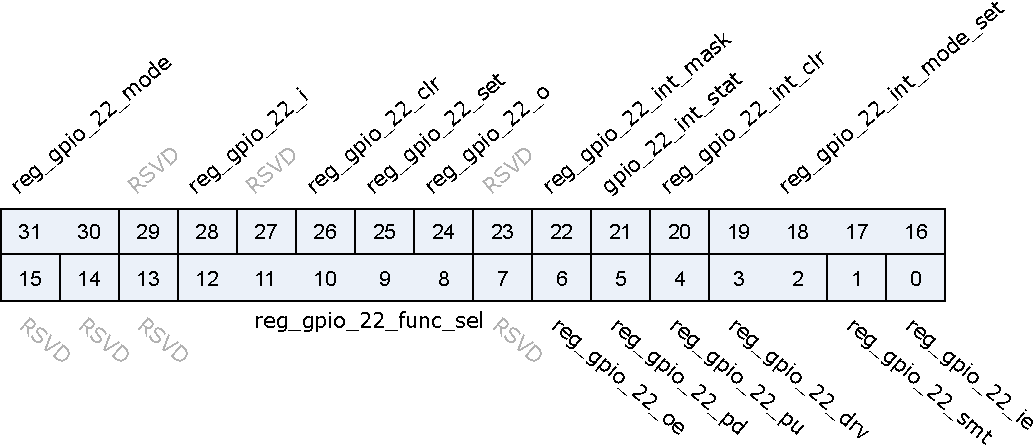
\includegraphics{glb_gpio_cfg22.pdf}
\end{figure}

\regdes{31:30&reg\_gpio\_22\_mode&r/w&0&When GPIO Function Selected to SWGPIO  \par 00 (Output Value Mode): GPIO Output by reg\_gpio\_x\_o Value  \par 01 (Set/Celar Mode     ) :GPIO Output set by reg\_gpio\_x\_set and clear by reg\_gpio\_x\_clr \par 10 : SWGPIO Source comes from  GPIO DMA (GPIO DMA Mode), GPIO Output value by gpio\_dma\_o \par 11: SWGPIO Source comes from  GPIO DMA (GPIO DMA Mode), GPIO Outout value by gpio\_dma\_set/gpio\_dma\_clr
\\\hline
29&RSVD& & & \\\hline
28&reg\_gpio\_22\_i&r&0&\\\hline
27&RSVD& & & \\\hline
26&reg\_gpio\_22\_clr&w1p&0&When SWGPIO @ Set/Clear Mode \par Set this bit will clear GPIO output value to 0,when set/clr at the same time, only set take effect
\\\hline
25&reg\_gpio\_22\_set&w1p&0&When SWGPIO @ Set/Clear Mode \par Set this bit will set GPIO output value to 1,when set/clr at the same time, only set take effect
\\\hline
24&reg\_gpio\_22\_o&r/w&0&When SWGPIO @ Output Value Mode \par 00 : GPIO Value changes according to this value \par 01 : GPIO Value Set by this register and clr by clr\_reg
\\\hline
23&RSVD& & & \\\hline
22&reg\_gpio\_22\_int\_mask&r/w&1&mask interrupt (1)\\\hline
21&gpio\_22\_int\_stat&r&0&interrupt status\\\hline
20&reg\_gpio\_22\_int\_clr&r/w&0&clear interrupt\\\hline
19:16&reg\_gpio\_22\_int\_mode\_set&r/w&0&0000 : sync falling edge trigger \par 0001 : sync rising edge trigger \par 0010 : sync low level trigger \par 0011 : sync high level trigger \par 01xx : sync rising \& falling edge trigger \par 1000 : async falling edge trigger \par 1001 : async rising edge trigger \par 1010 : async low level trigger \par 1011 : async high level trigger
\\\hline
15:13&RSVD& & & \\\hline
12:8&reg\_gpio\_22\_func\_sel&r/w&5'hB&GPIO Function Select (Default : SW-GPIO)\\\hline
7&RSVD& & & \\\hline
6&reg\_gpio\_22\_oe&r/w&0&Register Controlled GPIO Output Enable (Used when GPIO Function select to Register Control GPIO)\\\hline
5&reg\_gpio\_22\_pd&r/w&0&GPIO Pull Down Control\\\hline
4&reg\_gpio\_22\_pu&r/w&0&GPIO Pull Up Control\\\hline
3:2&reg\_gpio\_22\_drv&r/w&0&GPIO Driving Control\\\hline
1&reg\_gpio\_22\_smt&r/w&1&GPIO SMT Control\\\hline
0&reg\_gpio\_22\_ie&r/w&0&GPIO Input Enable\\\hline

}
\subsection{gpio\_cfg23}
\label{glb-gpio-cfg23}
地址:0x20000920
 \begin{figure}[H]
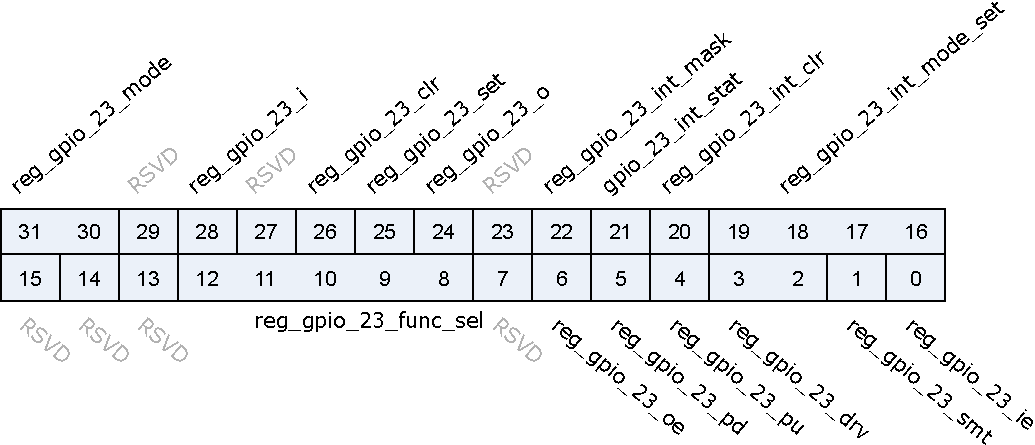
\includegraphics{glb_gpio_cfg23.pdf}
\end{figure}

\regdes{31:30&reg\_gpio\_23\_mode&r/w&0&When GPIO Function Selected to SWGPIO  \par 00 (Output Value Mode): GPIO Output by reg\_gpio\_x\_o Value  \par 01 (Set/Celar Mode     ) :GPIO Output set by reg\_gpio\_x\_set and clear by reg\_gpio\_x\_clr \par 10 : SWGPIO Source comes from  GPIO DMA (GPIO DMA Mode), GPIO Output value by gpio\_dma\_o \par 11: SWGPIO Source comes from  GPIO DMA (GPIO DMA Mode), GPIO Outout value by gpio\_dma\_set/gpio\_dma\_clr
\\\hline
29&RSVD& & & \\\hline
28&reg\_gpio\_23\_i&r&0&\\\hline
27&RSVD& & & \\\hline
26&reg\_gpio\_23\_clr&w1p&0&When SWGPIO @ Set/Clear Mode \par Set this bit will clear GPIO output value to 0,when set/clr at the same time, only set take effect
\\\hline
25&reg\_gpio\_23\_set&w1p&0&When SWGPIO @ Set/Clear Mode \par Set this bit will set GPIO output value to 1,when set/clr at the same time, only set take effect
\\\hline
24&reg\_gpio\_23\_o&r/w&0&When SWGPIO @ Output Value Mode \par 00 : GPIO Value changes according to this value \par 01 : GPIO Value Set by this register and clr by clr\_reg
\\\hline
23&RSVD& & & \\\hline
22&reg\_gpio\_23\_int\_mask&r/w&1&mask interrupt (1)\\\hline
21&gpio\_23\_int\_stat&r&0&interrupt status\\\hline
20&reg\_gpio\_23\_int\_clr&r/w&0&clear interrupt\\\hline
19:16&reg\_gpio\_23\_int\_mode\_set&r/w&0&0000 : sync falling edge trigger \par 0001 : sync rising edge trigger \par 0010 : sync low level trigger \par 0011 : sync high level trigger \par 01xx : sync rising \& falling edge trigger \par 1000 : async falling edge trigger \par 1001 : async rising edge trigger \par 1010 : async low level trigger \par 1011 : async high level trigger
\\\hline
15:13&RSVD& & & \\\hline
12:8&reg\_gpio\_23\_func\_sel&r/w&5'hB&GPIO Function Select (Default : SW-GPIO)\\\hline
7&RSVD& & & \\\hline
6&reg\_gpio\_23\_oe&r/w&0&Register Controlled GPIO Output Enable (Used when GPIO Function select to Register Control GPIO)\\\hline
5&reg\_gpio\_23\_pd&r/w&0&GPIO Pull Down Control\\\hline
4&reg\_gpio\_23\_pu&r/w&0&GPIO Pull Up Control\\\hline
3:2&reg\_gpio\_23\_drv&r/w&0&GPIO Driving Control\\\hline
1&reg\_gpio\_23\_smt&r/w&1&GPIO SMT Control\\\hline
0&reg\_gpio\_23\_ie&r/w&0&GPIO Input Enable\\\hline

}
\subsection{gpio\_cfg24}
\label{glb-gpio-cfg24}
地址:0x20000924
 \begin{figure}[H]
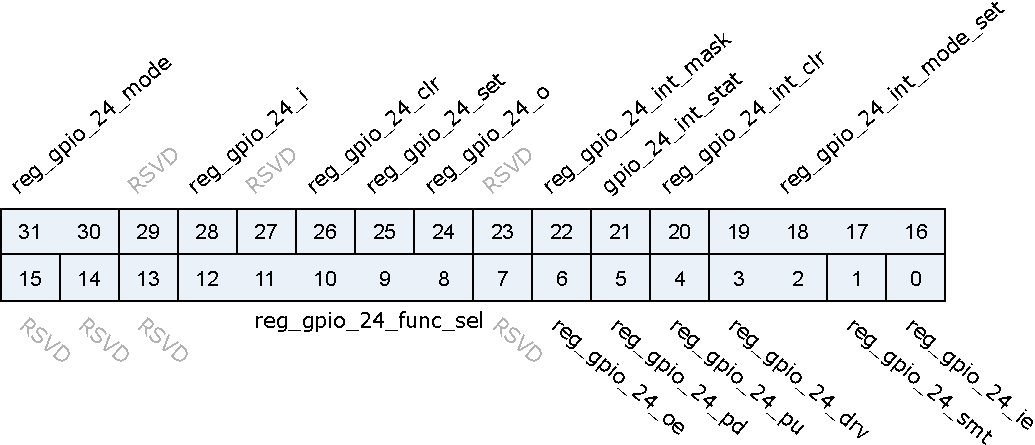
\includegraphics{glb_gpio_cfg24.pdf}
\end{figure}

\regdes{31:30&reg\_gpio\_24\_mode&r/w&0&When GPIO Function Selected to SWGPIO  \par 00 (Output Value Mode): GPIO Output by reg\_gpio\_x\_o Value  \par 01 (Set/Celar Mode     ) :GPIO Output set by reg\_gpio\_x\_set and clear by reg\_gpio\_x\_clr \par 10 : SWGPIO Source comes from  GPIO DMA (GPIO DMA Mode), GPIO Output value by gpio\_dma\_o \par 11: SWGPIO Source comes from  GPIO DMA (GPIO DMA Mode), GPIO Outout value by gpio\_dma\_set/gpio\_dma\_clr
\\\hline
29&RSVD& & & \\\hline
28&reg\_gpio\_24\_i&r&0&\\\hline
27&RSVD& & & \\\hline
26&reg\_gpio\_24\_clr&w1p&0&When SWGPIO @ Set/Clear Mode \par Set this bit will clear GPIO output value to 0,when set/clr at the same time, only set take effect
\\\hline
25&reg\_gpio\_24\_set&w1p&0&When SWGPIO @ Set/Clear Mode \par Set this bit will set GPIO output value to 1,when set/clr at the same time, only set take effect
\\\hline
24&reg\_gpio\_24\_o&r/w&0&When SWGPIO @ Output Value Mode \par 00 : GPIO Value changes according to this value \par 01 : GPIO Value Set by this register and clr by clr\_reg
\\\hline
23&RSVD& & & \\\hline
22&reg\_gpio\_24\_int\_mask&r/w&1&mask interrupt (1)\\\hline
21&gpio\_24\_int\_stat&r&0&interrupt status\\\hline
20&reg\_gpio\_24\_int\_clr&r/w&0&clear interrupt\\\hline
19:16&reg\_gpio\_24\_int\_mode\_set&r/w&0&0000 : sync falling edge trigger \par 0001 : sync rising edge trigger \par 0010 : sync low level trigger \par 0011 : sync high level trigger \par 01xx : sync rising \& falling edge trigger \par 1000 : async falling edge trigger \par 1001 : async rising edge trigger \par 1010 : async low level trigger \par 1011 : async high level trigger
\\\hline
15:13&RSVD& & & \\\hline
12:8&reg\_gpio\_24\_func\_sel&r/w&5'hB&GPIO Function Select (Default : SW-GPIO)\\\hline
7&RSVD& & & \\\hline
6&reg\_gpio\_24\_oe&r/w&0&Register Controlled GPIO Output Enable (Used when GPIO Function select to Register Control GPIO)\\\hline
5&reg\_gpio\_24\_pd&r/w&0&GPIO Pull Down Control\\\hline
4&reg\_gpio\_24\_pu&r/w&0&GPIO Pull Up Control\\\hline
3:2&reg\_gpio\_24\_drv&r/w&0&GPIO Driving Control\\\hline
1&reg\_gpio\_24\_smt&r/w&1&GPIO SMT Control\\\hline
0&reg\_gpio\_24\_ie&r/w&0&GPIO Input Enable\\\hline

}
\subsection{gpio\_cfg25}
\label{glb-gpio-cfg25}
地址:0x20000928
 \begin{figure}[H]
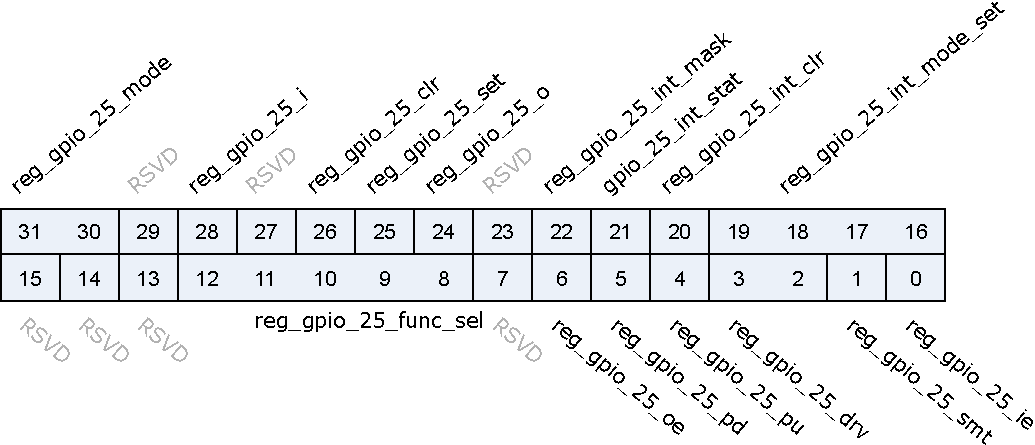
\includegraphics{glb_gpio_cfg25.pdf}
\end{figure}

\regdes{31:30&reg\_gpio\_25\_mode&r/w&0&When GPIO Function Selected to SWGPIO  \par 00 (Output Value Mode): GPIO Output by reg\_gpio\_x\_o Value  \par 01 (Set/Celar Mode     ) :GPIO Output set by reg\_gpio\_x\_set and clear by reg\_gpio\_x\_clr \par 10 : SWGPIO Source comes from  GPIO DMA (GPIO DMA Mode), GPIO Output value by gpio\_dma\_o \par 11: SWGPIO Source comes from  GPIO DMA (GPIO DMA Mode), GPIO Outout value by gpio\_dma\_set/gpio\_dma\_clr
\\\hline
29&RSVD& & & \\\hline
28&reg\_gpio\_25\_i&r&0&\\\hline
27&RSVD& & & \\\hline
26&reg\_gpio\_25\_clr&w1p&0&When SWGPIO @ Set/Clear Mode \par Set this bit will clear GPIO output value to 0,when set/clr at the same time, only set take effect
\\\hline
25&reg\_gpio\_25\_set&w1p&0&When SWGPIO @ Set/Clear Mode \par Set this bit will set GPIO output value to 1,when set/clr at the same time, only set take effect
\\\hline
24&reg\_gpio\_25\_o&r/w&0&When SWGPIO @ Output Value Mode \par 00 : GPIO Value changes according to this value \par 01 : GPIO Value Set by this register and clr by clr\_reg
\\\hline
23&RSVD& & & \\\hline
22&reg\_gpio\_25\_int\_mask&r/w&1&mask interrupt (1)\\\hline
21&gpio\_25\_int\_stat&r&0&interrupt status\\\hline
20&reg\_gpio\_25\_int\_clr&r/w&0&clear interrupt\\\hline
19:16&reg\_gpio\_25\_int\_mode\_set&r/w&0&0000 : sync falling edge trigger \par 0001 : sync rising edge trigger \par 0010 : sync low level trigger \par 0011 : sync high level trigger \par 01xx : sync rising \& falling edge trigger \par 1000 : async falling edge trigger \par 1001 : async rising edge trigger \par 1010 : async low level trigger \par 1011 : async high level trigger
\\\hline
15:13&RSVD& & & \\\hline
12:8&reg\_gpio\_25\_func\_sel&r/w&5'hB&GPIO Function Select (Default : SW-GPIO)\\\hline
7&RSVD& & & \\\hline
6&reg\_gpio\_25\_oe&r/w&0&Register Controlled GPIO Output Enable (Used when GPIO Function select to Register Control GPIO)\\\hline
5&reg\_gpio\_25\_pd&r/w&0&GPIO Pull Down Control\\\hline
4&reg\_gpio\_25\_pu&r/w&0&GPIO Pull Up Control\\\hline
3:2&reg\_gpio\_25\_drv&r/w&0&GPIO Driving Control\\\hline
1&reg\_gpio\_25\_smt&r/w&1&GPIO SMT Control\\\hline
0&reg\_gpio\_25\_ie&r/w&0&GPIO Input Enable\\\hline

}
\subsection{gpio\_cfg26}
\label{glb-gpio-cfg26}
地址:0x2000092c
 \begin{figure}[H]
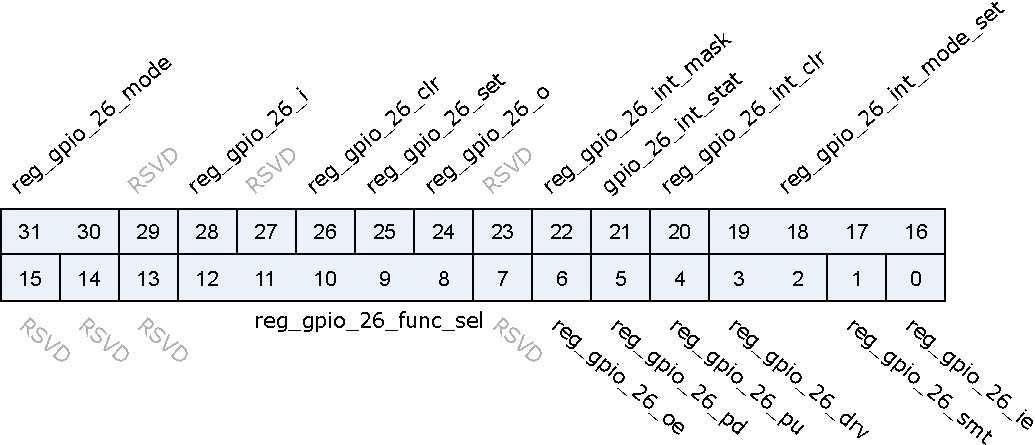
\includegraphics{glb_gpio_cfg26.pdf}
\end{figure}

\regdes{31:30&reg\_gpio\_26\_mode&r/w&0&When GPIO Function Selected to SWGPIO  \par 00 (Output Value Mode): GPIO Output by reg\_gpio\_x\_o Value  \par 01 (Set/Celar Mode     ) :GPIO Output set by reg\_gpio\_x\_set and clear by reg\_gpio\_x\_clr \par 10 : SWGPIO Source comes from  GPIO DMA (GPIO DMA Mode), GPIO Output value by gpio\_dma\_o \par 11: SWGPIO Source comes from  GPIO DMA (GPIO DMA Mode), GPIO Outout value by gpio\_dma\_set/gpio\_dma\_clr
\\\hline
29&RSVD& & & \\\hline
28&reg\_gpio\_26\_i&r&0&\\\hline
27&RSVD& & & \\\hline
26&reg\_gpio\_26\_clr&w1p&0&When SWGPIO @ Set/Clear Mode \par Set this bit will clear GPIO output value to 0,when set/clr at the same time, only set take effect
\\\hline
25&reg\_gpio\_26\_set&w1p&0&When SWGPIO @ Set/Clear Mode \par Set this bit will set GPIO output value to 1,when set/clr at the same time, only set take effect
\\\hline
24&reg\_gpio\_26\_o&r/w&0&When SWGPIO @ Output Value Mode \par 00 : GPIO Value changes according to this value \par 01 : GPIO Value Set by this register and clr by clr\_reg
\\\hline
23&RSVD& & & \\\hline
22&reg\_gpio\_26\_int\_mask&r/w&1&mask interrupt (1)\\\hline
21&gpio\_26\_int\_stat&r&0&interrupt status\\\hline
20&reg\_gpio\_26\_int\_clr&r/w&0&clear interrupt\\\hline
19:16&reg\_gpio\_26\_int\_mode\_set&r/w&0&0000 : sync falling edge trigger \par 0001 : sync rising edge trigger \par 0010 : sync low level trigger \par 0011 : sync high level trigger \par 01xx : sync rising \& falling edge trigger \par 1000 : async falling edge trigger \par 1001 : async rising edge trigger \par 1010 : async low level trigger \par 1011 : async high level trigger
\\\hline
15:13&RSVD& & & \\\hline
12:8&reg\_gpio\_26\_func\_sel&r/w&5'hB&GPIO Function Select (Default : SW-GPIO)\\\hline
7&RSVD& & & \\\hline
6&reg\_gpio\_26\_oe&r/w&0&Register Controlled GPIO Output Enable (Used when GPIO Function select to Register Control GPIO)\\\hline
5&reg\_gpio\_26\_pd&r/w&0&GPIO Pull Down Control\\\hline
4&reg\_gpio\_26\_pu&r/w&0&GPIO Pull Up Control\\\hline
3:2&reg\_gpio\_26\_drv&r/w&0&GPIO Driving Control\\\hline
1&reg\_gpio\_26\_smt&r/w&1&GPIO SMT Control\\\hline
0&reg\_gpio\_26\_ie&r/w&0&GPIO Input Enable\\\hline

}
\subsection{gpio\_cfg27}
\label{glb-gpio-cfg27}
地址:0x20000930
 \begin{figure}[H]
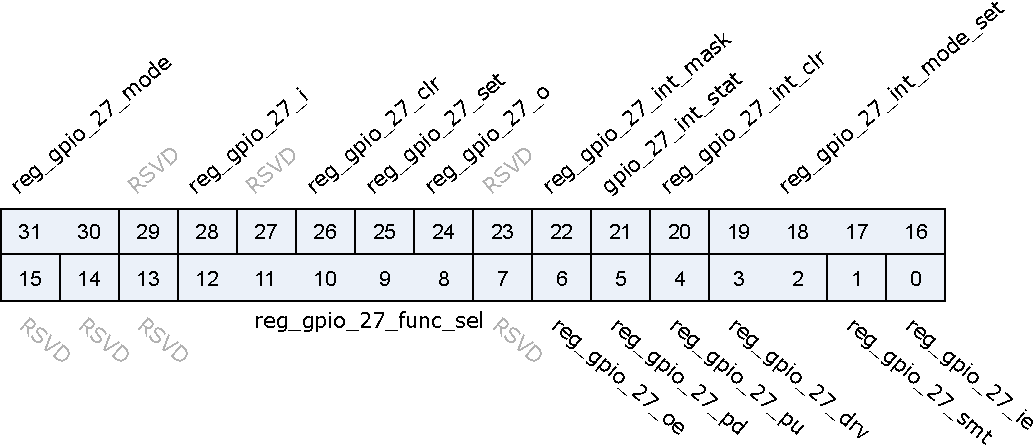
\includegraphics{glb_gpio_cfg27.pdf}
\end{figure}

\regdes{31:30&reg\_gpio\_27\_mode&r/w&0&When GPIO Function Selected to SWGPIO  \par 00 (Output Value Mode): GPIO Output by reg\_gpio\_x\_o Value  \par 01 (Set/Celar Mode     ) :GPIO Output set by reg\_gpio\_x\_set and clear by reg\_gpio\_x\_clr \par 10 : SWGPIO Source comes from  GPIO DMA (GPIO DMA Mode), GPIO Output value by gpio\_dma\_o \par 11: SWGPIO Source comes from  GPIO DMA (GPIO DMA Mode), GPIO Outout value by gpio\_dma\_set/gpio\_dma\_clr
\\\hline
29&RSVD& & & \\\hline
28&reg\_gpio\_27\_i&r&0&\\\hline
27&RSVD& & & \\\hline
26&reg\_gpio\_27\_clr&w1p&0&When SWGPIO @ Set/Clear Mode \par Set this bit will clear GPIO output value to 0,when set/clr at the same time, only set take effect
\\\hline
25&reg\_gpio\_27\_set&w1p&0&When SWGPIO @ Set/Clear Mode \par Set this bit will set GPIO output value to 1,when set/clr at the same time, only set take effect
\\\hline
24&reg\_gpio\_27\_o&r/w&0&When SWGPIO @ Output Value Mode \par 00 : GPIO Value changes according to this value \par 01 : GPIO Value Set by this register and clr by clr\_reg
\\\hline
23&RSVD& & & \\\hline
22&reg\_gpio\_27\_int\_mask&r/w&1&mask interrupt (1)\\\hline
21&gpio\_27\_int\_stat&r&0&interrupt status\\\hline
20&reg\_gpio\_27\_int\_clr&r/w&0&clear interrupt\\\hline
19:16&reg\_gpio\_27\_int\_mode\_set&r/w&0&0000 : sync falling edge trigger \par 0001 : sync rising edge trigger \par 0010 : sync low level trigger \par 0011 : sync high level trigger \par 01xx : sync rising \& falling edge trigger \par 1000 : async falling edge trigger \par 1001 : async rising edge trigger \par 1010 : async low level trigger \par 1011 : async high level trigger
\\\hline
15:13&RSVD& & & \\\hline
12:8&reg\_gpio\_27\_func\_sel&r/w&5'hB&GPIO Function Select (Default : SW-GPIO)\\\hline
7&RSVD& & & \\\hline
6&reg\_gpio\_27\_oe&r/w&0&Register Controlled GPIO Output Enable (Used when GPIO Function select to Register Control GPIO)\\\hline
5&reg\_gpio\_27\_pd&r/w&0&GPIO Pull Down Control\\\hline
4&reg\_gpio\_27\_pu&r/w&0&GPIO Pull Up Control\\\hline
3:2&reg\_gpio\_27\_drv&r/w&0&GPIO Driving Control\\\hline
1&reg\_gpio\_27\_smt&r/w&1&GPIO SMT Control\\\hline
0&reg\_gpio\_27\_ie&r/w&0&GPIO Input Enable\\\hline

}
\subsection{gpio\_cfg28}
\label{glb-gpio-cfg28}
地址:0x20000934
 \begin{figure}[H]
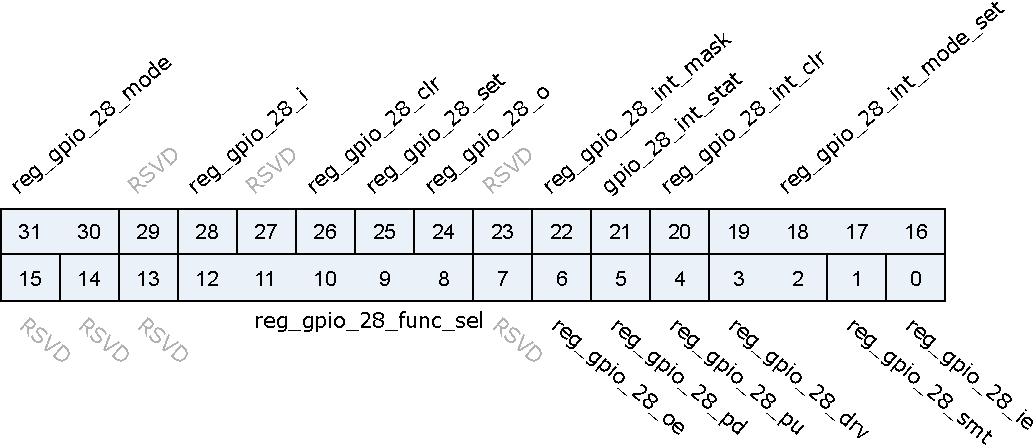
\includegraphics{glb_gpio_cfg28.pdf}
\end{figure}

\regdes{31:30&reg\_gpio\_28\_mode&r/w&0&When GPIO Function Selected to SWGPIO  \par 00 (Output Value Mode): GPIO Output by reg\_gpio\_x\_o Value  \par 01 (Set/Celar Mode     ) :GPIO Output set by reg\_gpio\_x\_set and clear by reg\_gpio\_x\_clr \par 10 : SWGPIO Source comes from  GPIO DMA (GPIO DMA Mode), GPIO Output value by gpio\_dma\_o \par 11: SWGPIO Source comes from  GPIO DMA (GPIO DMA Mode), GPIO Outout value by gpio\_dma\_set/gpio\_dma\_clr
\\\hline
29&RSVD& & & \\\hline
28&reg\_gpio\_28\_i&r&0&\\\hline
27&RSVD& & & \\\hline
26&reg\_gpio\_28\_clr&w1p&0&When SWGPIO @ Set/Clear Mode \par Set this bit will clear GPIO output value to 0,when set/clr at the same time, only set take effect
\\\hline
25&reg\_gpio\_28\_set&w1p&0&When SWGPIO @ Set/Clear Mode \par Set this bit will set GPIO output value to 1,when set/clr at the same time, only set take effect
\\\hline
24&reg\_gpio\_28\_o&r/w&0&When SWGPIO @ Output Value Mode \par 00 : GPIO Value changes according to this value \par 01 : GPIO Value Set by this register and clr by clr\_reg
\\\hline
23&RSVD& & & \\\hline
22&reg\_gpio\_28\_int\_mask&r/w&1&mask interrupt (1)\\\hline
21&gpio\_28\_int\_stat&r&0&interrupt status\\\hline
20&reg\_gpio\_28\_int\_clr&r/w&0&clear interrupt\\\hline
19:16&reg\_gpio\_28\_int\_mode\_set&r/w&0&0000 : sync falling edge trigger \par 0001 : sync rising edge trigger \par 0010 : sync low level trigger \par 0011 : sync high level trigger \par 01xx : sync rising \& falling edge trigger \par 1000 : async falling edge trigger \par 1001 : async rising edge trigger \par 1010 : async low level trigger \par 1011 : async high level trigger
\\\hline
15:13&RSVD& & & \\\hline
12:8&reg\_gpio\_28\_func\_sel&r/w&5'hB&GPIO Function Select (Default : SW-GPIO)\\\hline
7&RSVD& & & \\\hline
6&reg\_gpio\_28\_oe&r/w&0&Register Controlled GPIO Output Enable (Used when GPIO Function select to Register Control GPIO)\\\hline
5&reg\_gpio\_28\_pd&r/w&0&GPIO Pull Down Control\\\hline
4&reg\_gpio\_28\_pu&r/w&0&GPIO Pull Up Control\\\hline
3:2&reg\_gpio\_28\_drv&r/w&0&GPIO Driving Control\\\hline
1&reg\_gpio\_28\_smt&r/w&1&GPIO SMT Control\\\hline
0&reg\_gpio\_28\_ie&r/w&0&GPIO Input Enable\\\hline

}
\subsection{gpio\_cfg29}
\label{glb-gpio-cfg29}
地址:0x20000938
 \begin{figure}[H]
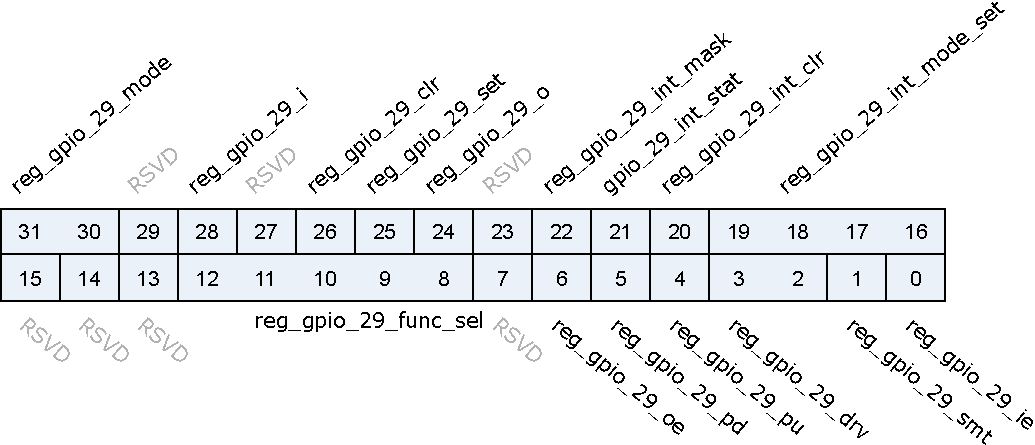
\includegraphics{glb_gpio_cfg29.pdf}
\end{figure}

\regdes{31:30&reg\_gpio\_29\_mode&r/w&0&When GPIO Function Selected to SWGPIO  \par 00 (Output Value Mode): GPIO Output by reg\_gpio\_x\_o Value  \par 01 (Set/Celar Mode     ) :GPIO Output set by reg\_gpio\_x\_set and clear by reg\_gpio\_x\_clr \par 10 : SWGPIO Source comes from  GPIO DMA (GPIO DMA Mode), GPIO Output value by gpio\_dma\_o \par 11: SWGPIO Source comes from  GPIO DMA (GPIO DMA Mode), GPIO Outout value by gpio\_dma\_set/gpio\_dma\_clr
\\\hline
29&RSVD& & & \\\hline
28&reg\_gpio\_29\_i&r&0&\\\hline
27&RSVD& & & \\\hline
26&reg\_gpio\_29\_clr&w1p&0&When SWGPIO @ Set/Clear Mode \par Set this bit will clear GPIO output value to 0,when set/clr at the same time, only set take effect
\\\hline
25&reg\_gpio\_29\_set&w1p&0&When SWGPIO @ Set/Clear Mode \par Set this bit will set GPIO output value to 1,when set/clr at the same time, only set take effect
\\\hline
24&reg\_gpio\_29\_o&r/w&0&When SWGPIO @ Output Value Mode \par 00 : GPIO Value changes according to this value \par 01 : GPIO Value Set by this register and clr by clr\_reg
\\\hline
23&RSVD& & & \\\hline
22&reg\_gpio\_29\_int\_mask&r/w&1&mask interrupt (1)\\\hline
21&gpio\_29\_int\_stat&r&0&interrupt status\\\hline
20&reg\_gpio\_29\_int\_clr&r/w&0&clear interrupt\\\hline
19:16&reg\_gpio\_29\_int\_mode\_set&r/w&0&0000 : sync falling edge trigger \par 0001 : sync rising edge trigger \par 0010 : sync low level trigger \par 0011 : sync high level trigger \par 01xx : sync rising \& falling edge trigger \par 1000 : async falling edge trigger \par 1001 : async rising edge trigger \par 1010 : async low level trigger \par 1011 : async high level trigger
\\\hline
15:13&RSVD& & & \\\hline
12:8&reg\_gpio\_29\_func\_sel&r/w&5'hB&GPIO Function Select (Default : SW-GPIO)\\\hline
7&RSVD& & & \\\hline
6&reg\_gpio\_29\_oe&r/w&0&Register Controlled GPIO Output Enable (Used when GPIO Function select to Register Control GPIO)\\\hline
5&reg\_gpio\_29\_pd&r/w&0&GPIO Pull Down Control\\\hline
4&reg\_gpio\_29\_pu&r/w&0&GPIO Pull Up Control\\\hline
3:2&reg\_gpio\_29\_drv&r/w&0&GPIO Driving Control\\\hline
1&reg\_gpio\_29\_smt&r/w&1&GPIO SMT Control\\\hline
0&reg\_gpio\_29\_ie&r/w&0&GPIO Input Enable\\\hline

}
\subsection{gpio\_cfg30}
\label{glb-gpio-cfg30}
地址:0x2000093c
 \begin{figure}[H]
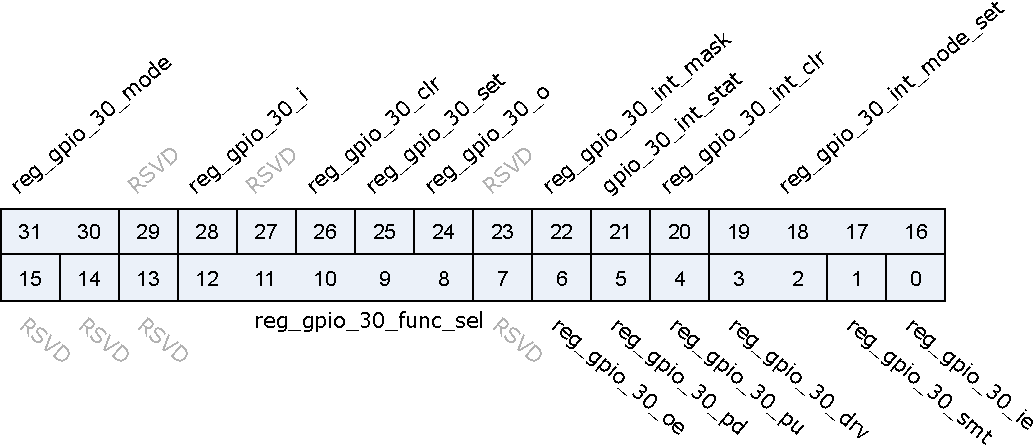
\includegraphics{glb_gpio_cfg30.pdf}
\end{figure}

\regdes{31:30&reg\_gpio\_30\_mode&r/w&0&When GPIO Function Selected to SWGPIO  \par 00 (Output Value Mode): GPIO Output by reg\_gpio\_x\_o Value  \par 01 (Set/Celar Mode     ) :GPIO Output set by reg\_gpio\_x\_set and clear by reg\_gpio\_x\_clr \par 10 : SWGPIO Source comes from  GPIO DMA (GPIO DMA Mode), GPIO Output value by gpio\_dma\_o \par 11: SWGPIO Source comes from  GPIO DMA (GPIO DMA Mode), GPIO Outout value by gpio\_dma\_set/gpio\_dma\_clr
\\\hline
29&RSVD& & & \\\hline
28&reg\_gpio\_30\_i&r&0&\\\hline
27&RSVD& & & \\\hline
26&reg\_gpio\_30\_clr&w1p&0&When SWGPIO @ Set/Clear Mode \par Set this bit will clear GPIO output value to 0,when set/clr at the same time, only set take effect
\\\hline
25&reg\_gpio\_30\_set&w1p&0&When SWGPIO @ Set/Clear Mode \par Set this bit will set GPIO output value to 1,when set/clr at the same time, only set take effect
\\\hline
24&reg\_gpio\_30\_o&r/w&0&When SWGPIO @ Output Value Mode \par 00 : GPIO Value changes according to this value \par 01 : GPIO Value Set by this register and clr by clr\_reg
\\\hline
23&RSVD& & & \\\hline
22&reg\_gpio\_30\_int\_mask&r/w&1&mask interrupt (1)\\\hline
21&gpio\_30\_int\_stat&r&0&interrupt status\\\hline
20&reg\_gpio\_30\_int\_clr&r/w&0&clear interrupt\\\hline
19:16&reg\_gpio\_30\_int\_mode\_set&r/w&0&0000 : sync falling edge trigger \par 0001 : sync rising edge trigger \par 0010 : sync low level trigger \par 0011 : sync high level trigger \par 01xx : sync rising \& falling edge trigger \par 1000 : async falling edge trigger \par 1001 : async rising edge trigger \par 1010 : async low level trigger \par 1011 : async high level trigger
\\\hline
15:13&RSVD& & & \\\hline
12:8&reg\_gpio\_30\_func\_sel&r/w&5'hB&GPIO Function Select (Default : SW-GPIO)\\\hline
7&RSVD& & & \\\hline
6&reg\_gpio\_30\_oe&r/w&0&Register Controlled GPIO Output Enable (Used when GPIO Function select to Register Control GPIO)\\\hline
5&reg\_gpio\_30\_pd&r/w&0&GPIO Pull Down Control\\\hline
4&reg\_gpio\_30\_pu&r/w&0&GPIO Pull Up Control\\\hline
3:2&reg\_gpio\_30\_drv&r/w&0&GPIO Driving Control\\\hline
1&reg\_gpio\_30\_smt&r/w&1&GPIO SMT Control\\\hline
0&reg\_gpio\_30\_ie&r/w&0&GPIO Input Enable\\\hline

}
\subsection{gpio\_cfg31}
\label{glb-gpio-cfg31}
地址:0x20000940
 \begin{figure}[H]
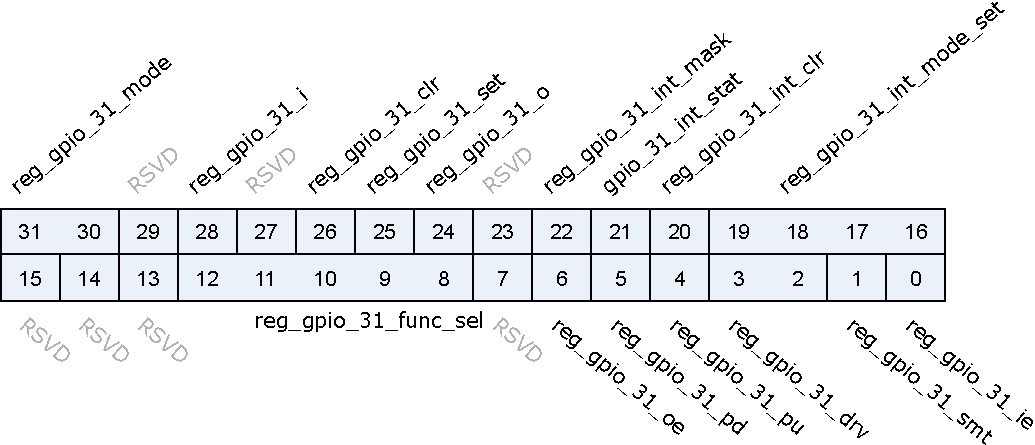
\includegraphics{glb_gpio_cfg31.pdf}
\end{figure}

\regdes{31:30&reg\_gpio\_31\_mode&r/w&0&When GPIO Function Selected to SWGPIO  \par 00 (Output Value Mode): GPIO Output by reg\_gpio\_x\_o Value  \par 01 (Set/Celar Mode     ) :GPIO Output set by reg\_gpio\_x\_set and clear by reg\_gpio\_x\_clr \par 10 : SWGPIO Source comes from  GPIO DMA (GPIO DMA Mode), GPIO Output value by gpio\_dma\_o \par 11: SWGPIO Source comes from  GPIO DMA (GPIO DMA Mode), GPIO Outout value by gpio\_dma\_set/gpio\_dma\_clr
\\\hline
29&RSVD& & & \\\hline
28&reg\_gpio\_31\_i&r&0&\\\hline
27&RSVD& & & \\\hline
26&reg\_gpio\_31\_clr&w1p&0&When SWGPIO @ Set/Clear Mode \par Set this bit will clear GPIO output value to 0,when set/clr at the same time, only set take effect
\\\hline
25&reg\_gpio\_31\_set&w1p&0&When SWGPIO @ Set/Clear Mode \par Set this bit will set GPIO output value to 1,when set/clr at the same time, only set take effect
\\\hline
24&reg\_gpio\_31\_o&r/w&0&When SWGPIO @ Output Value Mode \par 00 : GPIO Value changes according to this value \par 01 : GPIO Value Set by this register and clr by clr\_reg
\\\hline
23&RSVD& & & \\\hline
22&reg\_gpio\_31\_int\_mask&r/w&1&mask interrupt (1)\\\hline
21&gpio\_31\_int\_stat&r&0&interrupt status\\\hline
20&reg\_gpio\_31\_int\_clr&r/w&0&clear interrupt\\\hline
19:16&reg\_gpio\_31\_int\_mode\_set&r/w&0&0000 : sync falling edge trigger \par 0001 : sync rising edge trigger \par 0010 : sync low level trigger \par 0011 : sync high level trigger \par 01xx : sync rising \& falling edge trigger \par 1000 : async falling edge trigger \par 1001 : async rising edge trigger \par 1010 : async low level trigger \par 1011 : async high level trigger
\\\hline
15:13&RSVD& & & \\\hline
12:8&reg\_gpio\_31\_func\_sel&r/w&5'hB&GPIO Function Select (Default : SW-GPIO)\\\hline
7&RSVD& & & \\\hline
6&reg\_gpio\_31\_oe&r/w&0&Register Controlled GPIO Output Enable (Used when GPIO Function select to Register Control GPIO)\\\hline
5&reg\_gpio\_31\_pd&r/w&0&GPIO Pull Down Control\\\hline
4&reg\_gpio\_31\_pu&r/w&0&GPIO Pull Up Control\\\hline
3:2&reg\_gpio\_31\_drv&r/w&0&GPIO Driving Control\\\hline
1&reg\_gpio\_31\_smt&r/w&1&GPIO SMT Control\\\hline
0&reg\_gpio\_31\_ie&r/w&0&GPIO Input Enable\\\hline

}
\subsection{gpio\_cfg32}
\label{glb-gpio-cfg32}
地址:0x20000944
 \begin{figure}[H]
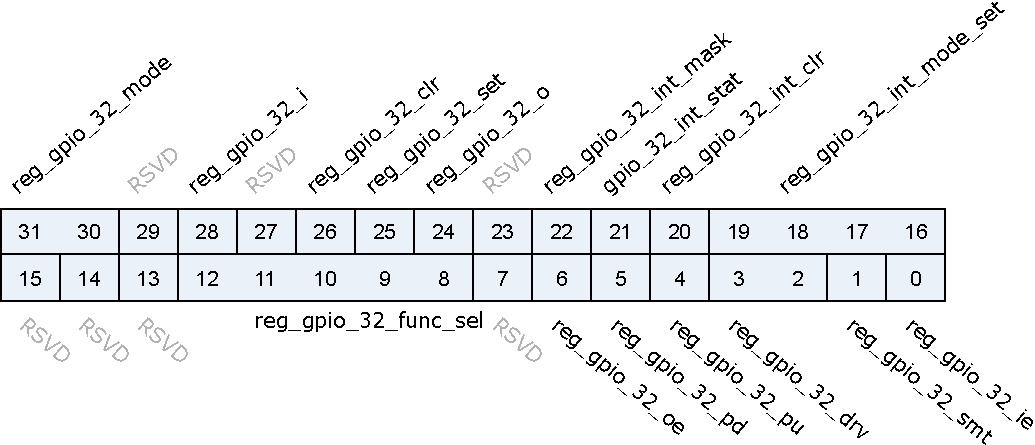
\includegraphics{glb_gpio_cfg32.pdf}
\end{figure}

\regdes{31:30&reg\_gpio\_32\_mode&r/w&0&When GPIO Function Selected to SWGPIO  \par 00 (Output Value Mode): GPIO Output by reg\_gpio\_x\_o Value  \par 01 (Set/Celar Mode     ) :GPIO Output set by reg\_gpio\_x\_set and clear by reg\_gpio\_x\_clr \par 10 : SWGPIO Source comes from  GPIO DMA (GPIO DMA Mode), GPIO Output value by gpio\_dma\_o \par 11: SWGPIO Source comes from  GPIO DMA (GPIO DMA Mode), GPIO Outout value by gpio\_dma\_set/gpio\_dma\_clr
\\\hline
29&RSVD& & & \\\hline
28&reg\_gpio\_32\_i&r&0&\\\hline
27&RSVD& & & \\\hline
26&reg\_gpio\_32\_clr&w1p&0&When SWGPIO @ Set/Clear Mode \par Set this bit will clear GPIO output value to 0,when set/clr at the same time, only set take effect
\\\hline
25&reg\_gpio\_32\_set&w1p&0&When SWGPIO @ Set/Clear Mode \par Set this bit will set GPIO output value to 1,when set/clr at the same time, only set take effect
\\\hline
24&reg\_gpio\_32\_o&r/w&0&When SWGPIO @ Output Value Mode \par 00 : GPIO Value changes according to this value \par 01 : GPIO Value Set by this register and clr by clr\_reg
\\\hline
23&RSVD& & & \\\hline
22&reg\_gpio\_32\_int\_mask&r/w&1&mask interrupt (1)\\\hline
21&gpio\_32\_int\_stat&r&0&interrupt status\\\hline
20&reg\_gpio\_32\_int\_clr&r/w&0&clear interrupt\\\hline
19:16&reg\_gpio\_32\_int\_mode\_set&r/w&0&0000 : sync falling edge trigger \par 0001 : sync rising edge trigger \par 0010 : sync low level trigger \par 0011 : sync high level trigger \par 01xx : sync rising \& falling edge trigger \par 1000 : async falling edge trigger \par 1001 : async rising edge trigger \par 1010 : async low level trigger \par 1011 : async high level trigger
\\\hline
15:13&RSVD& & & \\\hline
12:8&reg\_gpio\_32\_func\_sel&r/w&5'hB&GPIO Function Select (Default : SW-GPIO)\\\hline
7&RSVD& & & \\\hline
6&reg\_gpio\_32\_oe&r/w&0&Register Controlled GPIO Output Enable (Used when GPIO Function select to Register Control GPIO)\\\hline
5&reg\_gpio\_32\_pd&r/w&0&GPIO Pull Down Control\\\hline
4&reg\_gpio\_32\_pu&r/w&0&GPIO Pull Up Control\\\hline
3:2&reg\_gpio\_32\_drv&r/w&0&GPIO Driving Control\\\hline
1&reg\_gpio\_32\_smt&r/w&1&GPIO SMT Control\\\hline
0&reg\_gpio\_32\_ie&r/w&0&GPIO Input Enable\\\hline

}
\subsection{gpio\_cfg33}
\label{glb-gpio-cfg33}
地址:0x20000948
 \begin{figure}[H]
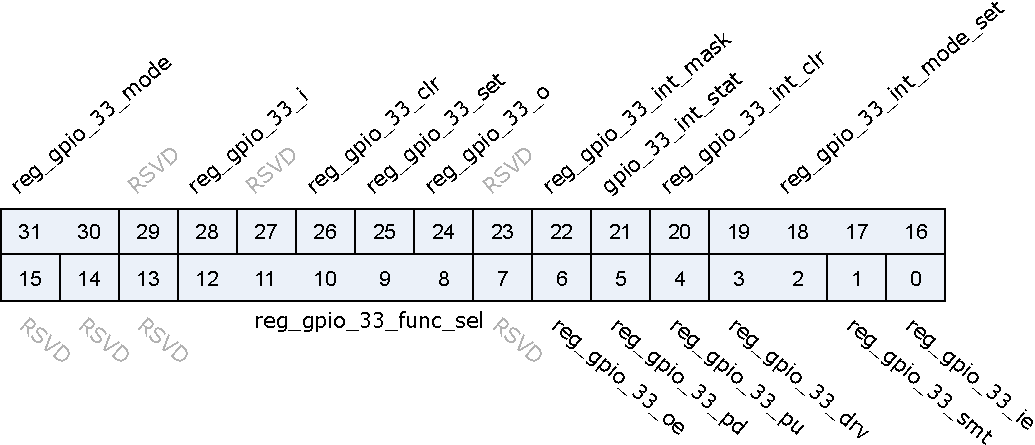
\includegraphics{glb_gpio_cfg33.pdf}
\end{figure}

\regdes{31:30&reg\_gpio\_33\_mode&r/w&0&When GPIO Function Selected to SWGPIO  \par 00 (Output Value Mode): GPIO Output by reg\_gpio\_x\_o Value  \par 01 (Set/Celar Mode     ) :GPIO Output set by reg\_gpio\_x\_set and clear by reg\_gpio\_x\_clr \par 10 : SWGPIO Source comes from  GPIO DMA (GPIO DMA Mode), GPIO Output value by gpio\_dma\_o \par 11: SWGPIO Source comes from  GPIO DMA (GPIO DMA Mode), GPIO Outout value by gpio\_dma\_set/gpio\_dma\_clr
\\\hline
29&RSVD& & & \\\hline
28&reg\_gpio\_33\_i&r&0&\\\hline
27&RSVD& & & \\\hline
26&reg\_gpio\_33\_clr&w1p&0&When SWGPIO @ Set/Clear Mode \par Set this bit will clear GPIO output value to 0,when set/clr at the same time, only set take effect
\\\hline
25&reg\_gpio\_33\_set&w1p&0&When SWGPIO @ Set/Clear Mode \par Set this bit will set GPIO output value to 1,when set/clr at the same time, only set take effect
\\\hline
24&reg\_gpio\_33\_o&r/w&0&When SWGPIO @ Output Value Mode \par 00 : GPIO Value changes according to this value \par 01 : GPIO Value Set by this register and clr by clr\_reg
\\\hline
23&RSVD& & & \\\hline
22&reg\_gpio\_33\_int\_mask&r/w&1&mask interrupt (1)\\\hline
21&gpio\_33\_int\_stat&r&0&interrupt status\\\hline
20&reg\_gpio\_33\_int\_clr&r/w&0&clear interrupt\\\hline
19:16&reg\_gpio\_33\_int\_mode\_set&r/w&0&0000 : sync falling edge trigger \par 0001 : sync rising edge trigger \par 0010 : sync low level trigger \par 0011 : sync high level trigger \par 01xx : sync rising \& falling edge trigger \par 1000 : async falling edge trigger \par 1001 : async rising edge trigger \par 1010 : async low level trigger \par 1011 : async high level trigger
\\\hline
15:13&RSVD& & & \\\hline
12:8&reg\_gpio\_33\_func\_sel&r/w&5'hB&GPIO Function Select (Default : SW-GPIO)\\\hline
7&RSVD& & & \\\hline
6&reg\_gpio\_33\_oe&r/w&0&Register Controlled GPIO Output Enable (Used when GPIO Function select to Register Control GPIO)\\\hline
5&reg\_gpio\_33\_pd&r/w&0&GPIO Pull Down Control\\\hline
4&reg\_gpio\_33\_pu&r/w&0&GPIO Pull Up Control\\\hline
3:2&reg\_gpio\_33\_drv&r/w&0&GPIO Driving Control\\\hline
1&reg\_gpio\_33\_smt&r/w&1&GPIO SMT Control\\\hline
0&reg\_gpio\_33\_ie&r/w&0&GPIO Input Enable\\\hline

}
\subsection{gpio\_cfg34}
\label{glb-gpio-cfg34}
地址:0x2000094c
 \begin{figure}[H]
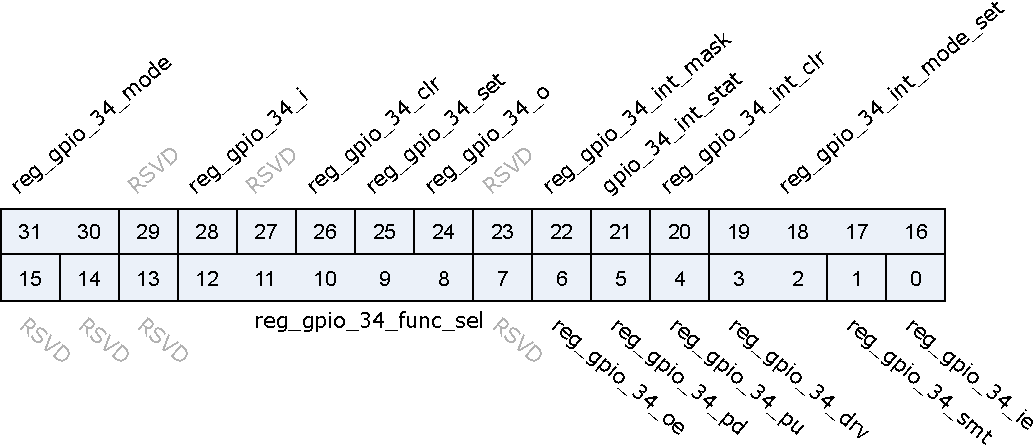
\includegraphics{glb_gpio_cfg34.pdf}
\end{figure}

\regdes{31:30&reg\_gpio\_34\_mode&r/w&0&When GPIO Function Selected to SWGPIO  \par 00 (Output Value Mode): GPIO Output by reg\_gpio\_x\_o Value  \par 01 (Set/Celar Mode     ) :GPIO Output set by reg\_gpio\_x\_set and clear by reg\_gpio\_x\_clr \par 10 : SWGPIO Source comes from  GPIO DMA (GPIO DMA Mode), GPIO Output value by gpio\_dma\_o \par 11: SWGPIO Source comes from  GPIO DMA (GPIO DMA Mode), GPIO Outout value by gpio\_dma\_set/gpio\_dma\_clr
\\\hline
29&RSVD& & & \\\hline
28&reg\_gpio\_34\_i&r&0&\\\hline
27&RSVD& & & \\\hline
26&reg\_gpio\_34\_clr&w1p&0&When SWGPIO @ Set/Clear Mode \par Set this bit will clear GPIO output value to 0,when set/clr at the same time, only set take effect
\\\hline
25&reg\_gpio\_34\_set&w1p&0&When SWGPIO @ Set/Clear Mode \par Set this bit will set GPIO output value to 1,when set/clr at the same time, only set take effect
\\\hline
24&reg\_gpio\_34\_o&r/w&0&When SWGPIO @ Output Value Mode \par 00 : GPIO Value changes according to this value \par 01 : GPIO Value Set by this register and clr by clr\_reg
\\\hline
23&RSVD& & & \\\hline
22&reg\_gpio\_34\_int\_mask&r/w&1&mask interrupt (1)\\\hline
21&gpio\_34\_int\_stat&r&0&interrupt status\\\hline
20&reg\_gpio\_34\_int\_clr&r/w&0&clear interrupt\\\hline
19:16&reg\_gpio\_34\_int\_mode\_set&r/w&0&0000 : sync falling edge trigger \par 0001 : sync rising edge trigger \par 0010 : sync low level trigger \par 0011 : sync high level trigger \par 01xx : sync rising \& falling edge trigger \par 1000 : async falling edge trigger \par 1001 : async rising edge trigger \par 1010 : async low level trigger \par 1011 : async high level trigger
\\\hline
15:13&RSVD& & & \\\hline
12:8&reg\_gpio\_34\_func\_sel&r/w&5'hB&GPIO Function Select (Default : SW-GPIO)\\\hline
7&RSVD& & & \\\hline
6&reg\_gpio\_34\_oe&r/w&0&Register Controlled GPIO Output Enable (Used when GPIO Function select to Register Control GPIO)\\\hline
5&reg\_gpio\_34\_pd&r/w&0&GPIO Pull Down Control\\\hline
4&reg\_gpio\_34\_pu&r/w&0&GPIO Pull Up Control\\\hline
3:2&reg\_gpio\_34\_drv&r/w&0&GPIO Driving Control\\\hline
1&reg\_gpio\_34\_smt&r/w&1&GPIO SMT Control\\\hline
0&reg\_gpio\_34\_ie&r/w&0&GPIO Input Enable\\\hline

}
\subsection{gpio\_cfg128}
\label{glb-gpio-cfg128}
地址:0x20000ac4
 \begin{figure}[H]
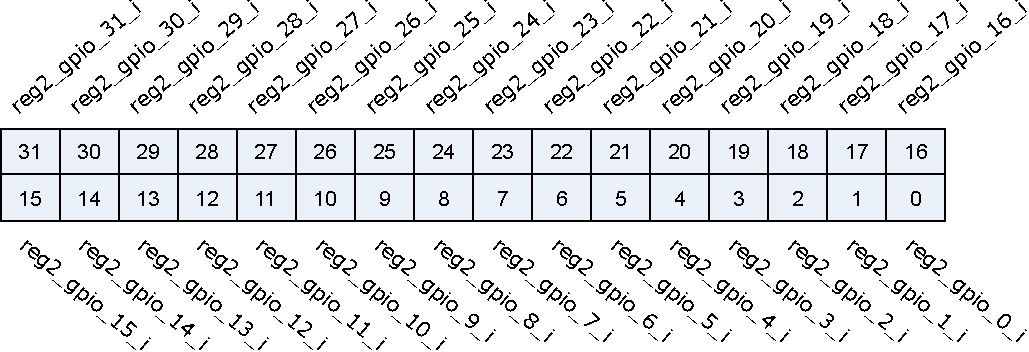
\includegraphics{glb_gpio_cfg128.pdf}
\end{figure}

\regdes{31&reg2\_gpio\_31\_i&r&0&Register Controlled GPIO Input value\\\hline
30&reg2\_gpio\_30\_i&r&0&Register Controlled GPIO Input value\\\hline
29&reg2\_gpio\_29\_i&r&0&Register Controlled GPIO Input value\\\hline
28&reg2\_gpio\_28\_i&r&0&Register Controlled GPIO Input value\\\hline
27&reg2\_gpio\_27\_i&r&0&Register Controlled GPIO Input value\\\hline
26&reg2\_gpio\_26\_i&r&0&Register Controlled GPIO Input value\\\hline
25&reg2\_gpio\_25\_i&r&0&Register Controlled GPIO Input value\\\hline
24&reg2\_gpio\_24\_i&r&0&Register Controlled GPIO Input value\\\hline
23&reg2\_gpio\_23\_i&r&0&Register Controlled GPIO Input value\\\hline
22&reg2\_gpio\_22\_i&r&0&Register Controlled GPIO Input value\\\hline
21&reg2\_gpio\_21\_i&r&0&Register Controlled GPIO Input value\\\hline
20&reg2\_gpio\_20\_i&r&0&Register Controlled GPIO Input value\\\hline
19&reg2\_gpio\_19\_i&r&0&Register Controlled GPIO Input value\\\hline
18&reg2\_gpio\_18\_i&r&0&Register Controlled GPIO Input value\\\hline
17&reg2\_gpio\_17\_i&r&0&Register Controlled GPIO Input value\\\hline
16&reg2\_gpio\_16\_i&r&0&Register Controlled GPIO Input value\\\hline
15&reg2\_gpio\_15\_i&r&0&Register Controlled GPIO Input value\\\hline
14&reg2\_gpio\_14\_i&r&0&Register Controlled GPIO Input value\\\hline
13&reg2\_gpio\_13\_i&r&0&Register Controlled GPIO Input value\\\hline
12&reg2\_gpio\_12\_i&r&0&Register Controlled GPIO Input value\\\hline
11&reg2\_gpio\_11\_i&r&0&Register Controlled GPIO Input value\\\hline
10&reg2\_gpio\_10\_i&r&0&Register Controlled GPIO Input value\\\hline
9&reg2\_gpio\_9\_i&r&0&Register Controlled GPIO Input value\\\hline
8&reg2\_gpio\_8\_i&r&0&Register Controlled GPIO Input value\\\hline
7&reg2\_gpio\_7\_i&r&0&Register Controlled GPIO Input value\\\hline
6&reg2\_gpio\_6\_i&r&0&Register Controlled GPIO Input value\\\hline
5&reg2\_gpio\_5\_i&r&0&Register Controlled GPIO Input value\\\hline
4&reg2\_gpio\_4\_i&r&0&Register Controlled GPIO Input value\\\hline
3&reg2\_gpio\_3\_i&r&0&Register Controlled GPIO Input value\\\hline
2&reg2\_gpio\_2\_i&r&0&Register Controlled GPIO Input value\\\hline
1&reg2\_gpio\_1\_i&r&0&Register Controlled GPIO Input value\\\hline
0&reg2\_gpio\_0\_i&r&0&Register Controlled GPIO Input value\\\hline

}
\subsection{gpio\_cfg129}
\label{glb-gpio-cfg129}
地址:0x20000ac8
 \begin{figure}[H]
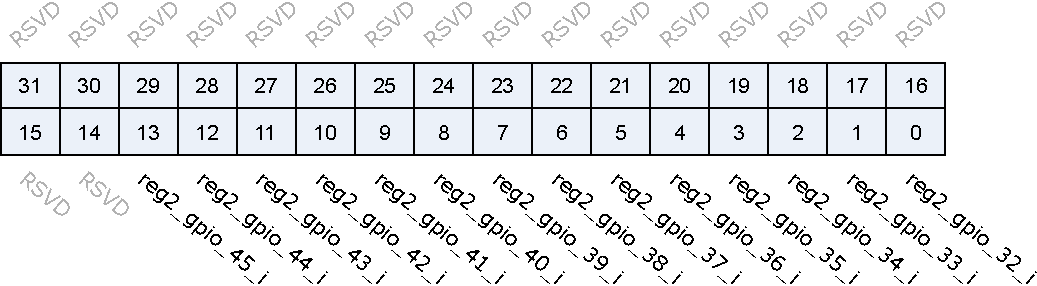
\includegraphics{glb_gpio_cfg129.pdf}
\end{figure}

\regdes{31:3&RSVD& & & \\\hline
2&reg2\_gpio\_34\_i&r&0&Register Controlled GPIO Input value\\\hline
1&reg2\_gpio\_33\_i&r&0&Register Controlled GPIO Input value\\\hline
0&reg2\_gpio\_32\_i&r&0&Register Controlled GPIO Input value\\\hline

}
\subsection{gpio\_cfg136}
\label{glb-gpio-cfg136}
地址:0x20000ae4
 \begin{figure}[H]
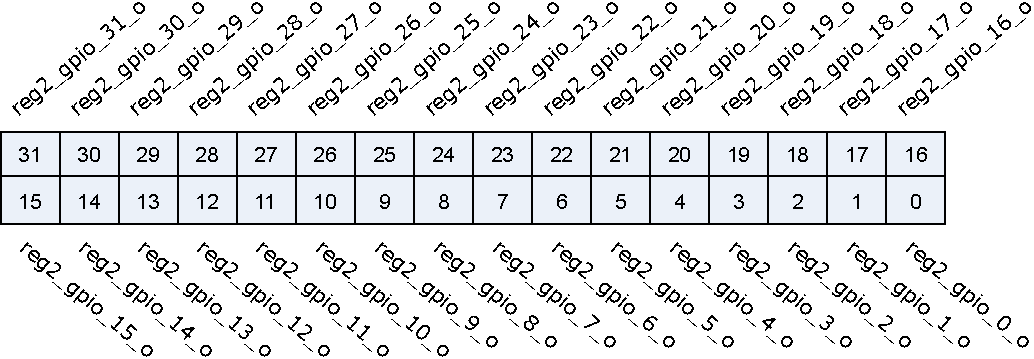
\includegraphics{glb_gpio_cfg136.pdf}
\end{figure}

\regdes{31&reg2\_gpio\_31\_o&r/w&0&Register Controlled GPIO Output Value\\\hline
30&reg2\_gpio\_30\_o&r/w&0&Register Controlled GPIO Output Value\\\hline
29&reg2\_gpio\_29\_o&r/w&0&Register Controlled GPIO Output Value\\\hline
28&reg2\_gpio\_28\_o&r/w&0&Register Controlled GPIO Output Value\\\hline
27&reg2\_gpio\_27\_o&r/w&0&Register Controlled GPIO Output Value\\\hline
26&reg2\_gpio\_26\_o&r/w&0&Register Controlled GPIO Output Value\\\hline
25&reg2\_gpio\_25\_o&r/w&0&Register Controlled GPIO Output Value\\\hline
24&reg2\_gpio\_24\_o&r/w&0&Register Controlled GPIO Output Value\\\hline
23&reg2\_gpio\_23\_o&r/w&0&Register Controlled GPIO Output Value\\\hline
22&reg2\_gpio\_22\_o&r/w&0&Register Controlled GPIO Output Value\\\hline
21&reg2\_gpio\_21\_o&r/w&0&Register Controlled GPIO Output Value\\\hline
20&reg2\_gpio\_20\_o&r/w&0&Register Controlled GPIO Output Value\\\hline
19&reg2\_gpio\_19\_o&r/w&0&Register Controlled GPIO Output Value\\\hline
18&reg2\_gpio\_18\_o&r/w&0&Register Controlled GPIO Output Value\\\hline
17&reg2\_gpio\_17\_o&r/w&0&Register Controlled GPIO Output Value\\\hline
16&reg2\_gpio\_16\_o&r/w&0&Register Controlled GPIO Output Value\\\hline
15&reg2\_gpio\_15\_o&r/w&0&Register Controlled GPIO Output Value\\\hline
14&reg2\_gpio\_14\_o&r/w&0&Register Controlled GPIO Output Value\\\hline
13&reg2\_gpio\_13\_o&r/w&0&Register Controlled GPIO Output Value\\\hline
12&reg2\_gpio\_12\_o&r/w&0&Register Controlled GPIO Output Value\\\hline
11&reg2\_gpio\_11\_o&r/w&0&Register Controlled GPIO Output Value\\\hline
10&reg2\_gpio\_10\_o&r/w&0&Register Controlled GPIO Output Value\\\hline
9&reg2\_gpio\_9\_o&r/w&0&Register Controlled GPIO Output Value\\\hline
8&reg2\_gpio\_8\_o&r/w&0&Register Controlled GPIO Output Value\\\hline
7&reg2\_gpio\_7\_o&r/w&0&Register Controlled GPIO Output Value\\\hline
6&reg2\_gpio\_6\_o&r/w&0&Register Controlled GPIO Output Value\\\hline
5&reg2\_gpio\_5\_o&r/w&0&Register Controlled GPIO Output Value\\\hline
4&reg2\_gpio\_4\_o&r/w&0&Register Controlled GPIO Output Value\\\hline
3&reg2\_gpio\_3\_o&r/w&0&Register Controlled GPIO Output Value\\\hline
2&reg2\_gpio\_2\_o&r/w&0&Register Controlled GPIO Output Value\\\hline
1&reg2\_gpio\_1\_o&r/w&0&Register Controlled GPIO Output Value\\\hline
0&reg2\_gpio\_0\_o&r/w&0&Register Controlled GPIO Output Value\\\hline

}
\subsection{gpio\_cfg137}
\label{glb-gpio-cfg137}
地址:0x20000ae8
 \begin{figure}[H]
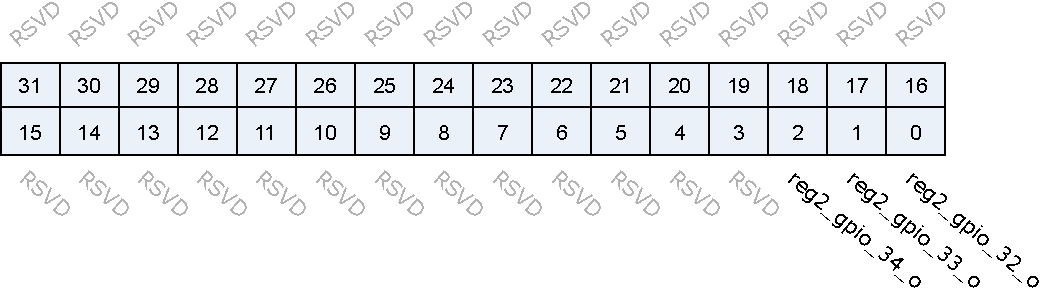
\includegraphics{glb_gpio_cfg137.pdf}
\end{figure}

\regdes{31:3&RSVD& & & \\\hline
2&reg2\_gpio\_34\_o&r/w&0&Register Controlled GPIO Output Value\\\hline
1&reg2\_gpio\_33\_o&r/w&0&Register Controlled GPIO Output Value\\\hline
0&reg2\_gpio\_32\_o&r/w&0&Register Controlled GPIO Output Value\\\hline

}
\subsection{gpio\_cfg138}
\label{glb-gpio-cfg138}
地址:0x20000aec
 \begin{figure}[H]
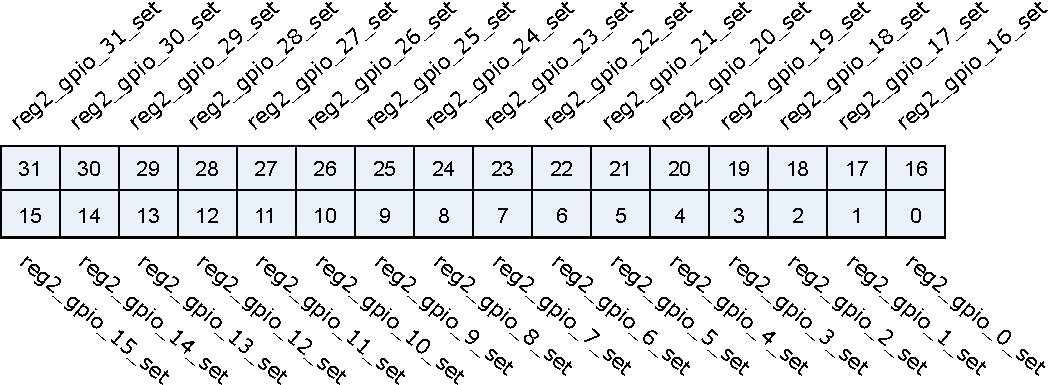
\includegraphics{glb_gpio_cfg138.pdf}
\end{figure}

\regdes{31&reg2\_gpio\_31\_set&w1p&0&When SWGPIO @ Set/Clear Mode \par Set this bit will set GPIO output value to 1,when set/clr at the same time, only set take effect
\\\hline
30&reg2\_gpio\_30\_set&w1p&0&When SWGPIO @ Set/Clear Mode \par Set this bit will set GPIO output value to 1,when set/clr at the same time, only set take effect
\\\hline
29&reg2\_gpio\_29\_set&w1p&0&When SWGPIO @ Set/Clear Mode \par Set this bit will set GPIO output value to 1,when set/clr at the same time, only set take effect
\\\hline
28&reg2\_gpio\_28\_set&w1p&0&When SWGPIO @ Set/Clear Mode \par Set this bit will set GPIO output value to 1,when set/clr at the same time, only set take effect
\\\hline
27&reg2\_gpio\_27\_set&w1p&0&When SWGPIO @ Set/Clear Mode \par Set this bit will set GPIO output value to 1,when set/clr at the same time, only set take effect
\\\hline
26&reg2\_gpio\_26\_set&w1p&0&When SWGPIO @ Set/Clear Mode \par Set this bit will set GPIO output value to 1,when set/clr at the same time, only set take effect
\\\hline
25&reg2\_gpio\_25\_set&w1p&0&When SWGPIO @ Set/Clear Mode \par Set this bit will set GPIO output value to 1,when set/clr at the same time, only set take effect
\\\hline
24&reg2\_gpio\_24\_set&w1p&0&When SWGPIO @ Set/Clear Mode \par Set this bit will set GPIO output value to 1,when set/clr at the same time, only set take effect
\\\hline
23&reg2\_gpio\_23\_set&w1p&0&When SWGPIO @ Set/Clear Mode \par Set this bit will set GPIO output value to 1,when set/clr at the same time, only set take effect
\\\hline
22&reg2\_gpio\_22\_set&w1p&0&When SWGPIO @ Set/Clear Mode \par Set this bit will set GPIO output value to 1,when set/clr at the same time, only set take effect
\\\hline
21&reg2\_gpio\_21\_set&w1p&0&When SWGPIO @ Set/Clear Mode \par Set this bit will set GPIO output value to 1,when set/clr at the same time, only set take effect
\\\hline
20&reg2\_gpio\_20\_set&w1p&0&When SWGPIO @ Set/Clear Mode \par Set this bit will set GPIO output value to 1,when set/clr at the same time, only set take effect
\\\hline
19&reg2\_gpio\_19\_set&w1p&0&When SWGPIO @ Set/Clear Mode \par Set this bit will set GPIO output value to 1,when set/clr at the same time, only set take effect
\\\hline
18&reg2\_gpio\_18\_set&w1p&0&When SWGPIO @ Set/Clear Mode \par Set this bit will set GPIO output value to 1,when set/clr at the same time, only set take effect
\\\hline
17&reg2\_gpio\_17\_set&w1p&0&When SWGPIO @ Set/Clear Mode \par Set this bit will set GPIO output value to 1,when set/clr at the same time, only set take effect
\\\hline
16&reg2\_gpio\_16\_set&w1p&0&When SWGPIO @ Set/Clear Mode \par Set this bit will set GPIO output value to 1,when set/clr at the same time, only set take effect
\\\hline
15&reg2\_gpio\_15\_set&w1p&0&When SWGPIO @ Set/Clear Mode \par Set this bit will set GPIO output value to 1,when set/clr at the same time, only set take effect
\\\hline
14&reg2\_gpio\_14\_set&w1p&0&When SWGPIO @ Set/Clear Mode \par Set this bit will set GPIO output value to 1,when set/clr at the same time, only set take effect
\\\hline
13&reg2\_gpio\_13\_set&w1p&0&When SWGPIO @ Set/Clear Mode \par Set this bit will set GPIO output value to 1,when set/clr at the same time, only set take effect
\\\hline
12&reg2\_gpio\_12\_set&w1p&0&When SWGPIO @ Set/Clear Mode \par Set this bit will set GPIO output value to 1,when set/clr at the same time, only set take effect
\\\hline
11&reg2\_gpio\_11\_set&w1p&0&When SWGPIO @ Set/Clear Mode \par Set this bit will set GPIO output value to 1,when set/clr at the same time, only set take effect
\\\hline
10&reg2\_gpio\_10\_set&w1p&0&When SWGPIO @ Set/Clear Mode \par Set this bit will set GPIO output value to 1,when set/clr at the same time, only set take effect
\\\hline
9&reg2\_gpio\_9\_set&w1p&0&When SWGPIO @ Set/Clear Mode \par Set this bit will set GPIO output value to 1,when set/clr at the same time, only set take effect
\\\hline
8&reg2\_gpio\_8\_set&w1p&0&When SWGPIO @ Set/Clear Mode \par Set this bit will set GPIO output value to 1,when set/clr at the same time, only set take effect
\\\hline
7&reg2\_gpio\_7\_set&w1p&0&When SWGPIO @ Set/Clear Mode \par Set this bit will set GPIO output value to 1,when set/clr at the same time, only set take effect
\\\hline
6&reg2\_gpio\_6\_set&w1p&0&When SWGPIO @ Set/Clear Mode \par Set this bit will set GPIO output value to 1,when set/clr at the same time, only set take effect
\\\hline
5&reg2\_gpio\_5\_set&w1p&0&When SWGPIO @ Set/Clear Mode \par Set this bit will set GPIO output value to 1,when set/clr at the same time, only set take effect
\\\hline
4&reg2\_gpio\_4\_set&w1p&0&When SWGPIO @ Set/Clear Mode \par Set this bit will set GPIO output value to 1,when set/clr at the same time, only set take effect
\\\hline
3&reg2\_gpio\_3\_set&w1p&0&When SWGPIO @ Set/Clear Mode \par Set this bit will set GPIO output value to 1,when set/clr at the same time, only set take effect
\\\hline
2&reg2\_gpio\_2\_set&w1p&0&When SWGPIO @ Set/Clear Mode \par Set this bit will set GPIO output value to 1,when set/clr at the same time, only set take effect
\\\hline
1&reg2\_gpio\_1\_set&w1p&0&When SWGPIO @ Set/Clear Mode \par Set this bit will set GPIO output value to 1,when set/clr at the same time, only set take effect
\\\hline
0&reg2\_gpio\_0\_set&w1p&0&When SWGPIO @ Set/Clear Mode \par Set this bit will set GPIO output value to 1,when set/clr at the same time, only set take effect
\\\hline

}
\subsection{gpio\_cfg139}
\label{glb-gpio-cfg139}
地址:0x20000af0
 \begin{figure}[H]
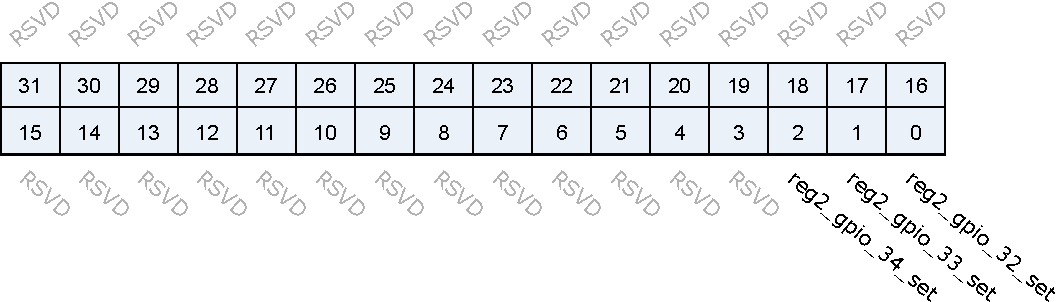
\includegraphics{glb_gpio_cfg139.pdf}
\end{figure}

\regdes{31:3&RSVD& & & \\\hline
2&reg2\_gpio\_34\_set&w1p&0&When SWGPIO @ Set/Clear Mode \par Set this bit will set GPIO output value to 1,when set/clr at the same time, only set take effect
\\\hline
1&reg2\_gpio\_33\_set&w1p&0&When SWGPIO @ Set/Clear Mode \par Set this bit will set GPIO output value to 1,when set/clr at the same time, only set take effect
\\\hline
0&reg2\_gpio\_32\_set&w1p&0&When SWGPIO @ Set/Clear Mode \par Set this bit will set GPIO output value to 1,when set/clr at the same time, only set take effect
\\\hline
-1:32&RSVD& & & \\\hline
31&reg2\_gpio\_31\_clr&w1p&0&When SWGPIO @ Set/Clear Mode \par Set this bit will clear GPIO output value to 0,when set/clr at the same time, only set take effect
\\\hline
30&reg2\_gpio\_30\_clr&w1p&0&When SWGPIO @ Set/Clear Mode \par Set this bit will clear GPIO output value to 0,when set/clr at the same time, only set take effect
\\\hline
29&reg2\_gpio\_29\_clr&w1p&0&When SWGPIO @ Set/Clear Mode \par Set this bit will clear GPIO output value to 0,when set/clr at the same time, only set take effect
\\\hline
28&reg2\_gpio\_28\_clr&w1p&0&When SWGPIO @ Set/Clear Mode \par Set this bit will clear GPIO output value to 0,when set/clr at the same time, only set take effect
\\\hline
27&reg2\_gpio\_27\_clr&w1p&0&When SWGPIO @ Set/Clear Mode \par Set this bit will clear GPIO output value to 0,when set/clr at the same time, only set take effect
\\\hline
26&reg2\_gpio\_26\_clr&w1p&0&When SWGPIO @ Set/Clear Mode \par Set this bit will clear GPIO output value to 0,when set/clr at the same time, only set take effect
\\\hline
25&reg2\_gpio\_25\_clr&w1p&0&When SWGPIO @ Set/Clear Mode \par Set this bit will clear GPIO output value to 0,when set/clr at the same time, only set take effect
\\\hline
24&reg2\_gpio\_24\_clr&w1p&0&When SWGPIO @ Set/Clear Mode \par Set this bit will clear GPIO output value to 0,when set/clr at the same time, only set take effect
\\\hline
23&reg2\_gpio\_23\_clr&w1p&0&When SWGPIO @ Set/Clear Mode \par Set this bit will clear GPIO output value to 0,when set/clr at the same time, only set take effect
\\\hline
22&reg2\_gpio\_22\_clr&w1p&0&When SWGPIO @ Set/Clear Mode \par Set this bit will clear GPIO output value to 0,when set/clr at the same time, only set take effect
\\\hline
21&reg2\_gpio\_21\_clr&w1p&0&When SWGPIO @ Set/Clear Mode \par Set this bit will clear GPIO output value to 0,when set/clr at the same time, only set take effect
\\\hline
20&reg2\_gpio\_20\_clr&w1p&0&When SWGPIO @ Set/Clear Mode \par Set this bit will clear GPIO output value to 0,when set/clr at the same time, only set take effect
\\\hline
19&reg2\_gpio\_19\_clr&w1p&0&When SWGPIO @ Set/Clear Mode \par Set this bit will clear GPIO output value to 0,when set/clr at the same time, only set take effect
\\\hline
18&reg2\_gpio\_18\_clr&w1p&0&When SWGPIO @ Set/Clear Mode \par Set this bit will clear GPIO output value to 0,when set/clr at the same time, only set take effect
\\\hline
17&reg2\_gpio\_17\_clr&w1p&0&When SWGPIO @ Set/Clear Mode \par Set this bit will clear GPIO output value to 0,when set/clr at the same time, only set take effect
\\\hline
16&reg2\_gpio\_16\_clr&w1p&0&When SWGPIO @ Set/Clear Mode \par Set this bit will clear GPIO output value to 0,when set/clr at the same time, only set take effect
\\\hline
15&reg2\_gpio\_15\_clr&w1p&0&When SWGPIO @ Set/Clear Mode \par Set this bit will clear GPIO output value to 0,when set/clr at the same time, only set take effect
\\\hline
14&reg2\_gpio\_14\_clr&w1p&0&When SWGPIO @ Set/Clear Mode \par Set this bit will clear GPIO output value to 0,when set/clr at the same time, only set take effect
\\\hline
13&reg2\_gpio\_13\_clr&w1p&0&When SWGPIO @ Set/Clear Mode \par Set this bit will clear GPIO output value to 0,when set/clr at the same time, only set take effect
\\\hline
12&reg2\_gpio\_12\_clr&w1p&0&When SWGPIO @ Set/Clear Mode \par Set this bit will clear GPIO output value to 0,when set/clr at the same time, only set take effect
\\\hline
11&reg2\_gpio\_11\_clr&w1p&0&When SWGPIO @ Set/Clear Mode \par Set this bit will clear GPIO output value to 0,when set/clr at the same time, only set take effect
\\\hline
10&reg2\_gpio\_10\_clr&w1p&0&When SWGPIO @ Set/Clear Mode \par Set this bit will clear GPIO output value to 0,when set/clr at the same time, only set take effect
\\\hline
9&reg2\_gpio\_9\_clr&w1p&0&When SWGPIO @ Set/Clear Mode \par Set this bit will clear GPIO output value to 0,when set/clr at the same time, only set take effect
\\\hline
8&reg2\_gpio\_8\_clr&w1p&0&When SWGPIO @ Set/Clear Mode \par Set this bit will clear GPIO output value to 0,when set/clr at the same time, only set take effect
\\\hline
7&reg2\_gpio\_7\_clr&w1p&0&When SWGPIO @ Set/Clear Mode \par Set this bit will clear GPIO output value to 0,when set/clr at the same time, only set take effect
\\\hline
6&reg2\_gpio\_6\_clr&w1p&0&When SWGPIO @ Set/Clear Mode \par Set this bit will clear GPIO output value to 0,when set/clr at the same time, only set take effect
\\\hline
5&reg2\_gpio\_5\_clr&w1p&0&When SWGPIO @ Set/Clear Mode \par Set this bit will clear GPIO output value to 0,when set/clr at the same time, only set take effect
\\\hline
4&reg2\_gpio\_4\_clr&w1p&0&When SWGPIO @ Set/Clear Mode \par Set this bit will clear GPIO output value to 0,when set/clr at the same time, only set take effect
\\\hline
3&reg2\_gpio\_3\_clr&w1p&0&When SWGPIO @ Set/Clear Mode \par Set this bit will clear GPIO output value to 0,when set/clr at the same time, only set take effect
\\\hline
2&reg2\_gpio\_2\_clr&w1p&0&When SWGPIO @ Set/Clear Mode \par Set this bit will clear GPIO output value to 0,when set/clr at the same time, only set take effect
\\\hline
1&reg2\_gpio\_1\_clr&w1p&0&When SWGPIO @ Set/Clear Mode \par Set this bit will clear GPIO output value to 0,when set/clr at the same time, only set take effect
\\\hline
0&reg2\_gpio\_0\_clr&w1p&0&When SWGPIO @ Set/Clear Mode \par Set this bit will clear GPIO output value to 0,when set/clr at the same time, only set take effect
\\\hline

}
\subsection{gpio\_cfg141}
\label{glb-gpio-cfg141}
地址:0x20000af8
 \begin{figure}[H]
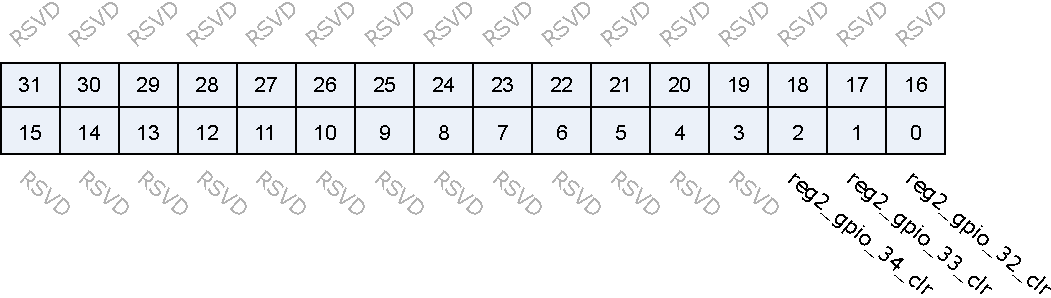
\includegraphics{glb_gpio_cfg141.pdf}
\end{figure}

\regdes{31:3&RSVD& & & \\\hline
2&reg2\_gpio\_34\_clr&w1p&0&When SWGPIO @ Set/Clear Mode \par Set this bit will clear GPIO output value to 0,when set/clr at the same time, only set take effect
\\\hline
1&reg2\_gpio\_33\_clr&w1p&0&When SWGPIO @ Set/Clear Mode \par Set this bit will clear GPIO output value to 0,when set/clr at the same time, only set take effect
\\\hline
0&reg2\_gpio\_32\_clr&w1p&0&When SWGPIO @ Set/Clear Mode \par Set this bit will clear GPIO output value to 0,when set/clr at the same time, only set take effect
\\\hline

}
\subsection{gpio\_cfg142}
\label{glb-gpio-cfg142}
地址:0x20000afc
 \begin{figure}[H]
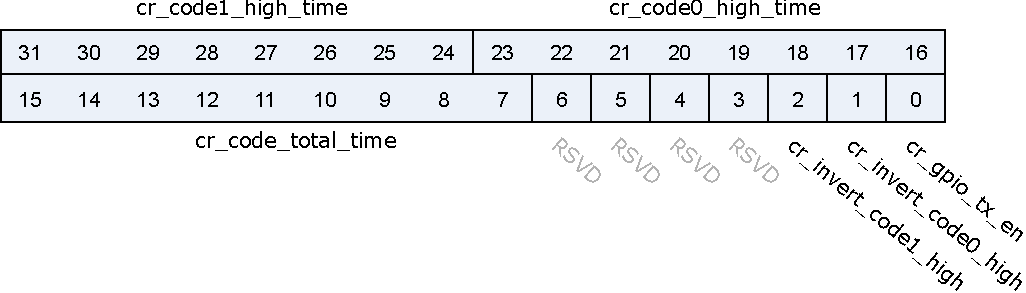
\includegraphics{glb_gpio_cfg142.pdf}
\end{figure}

\regdes{31:24&cr\_code1\_high\_time&r/w&8'd200&Used to generate Code 1  Duty Cycle Waveform (in units of xclk (XTAL or RC32M) clock cycle) \par waveform keep high during cr\_code1\_high\_time  \par waveform keep low  during cr\_code1\_low\_time (cr\_code\_total\_time - cr\_code1\_high\_time )
\\\hline
23:16&cr\_code0\_high\_time&r/w&8'd200&Used to generate Code 0  Duty Cycle Waveform (in units of xclk (XTAL or RC32M) clock cycle) \par waveform keep high during cr\_code0\_high\_time  \par waveform keep low  during cr\_code0\_low\_time (cr\_code\_total\_time - cr\_code0\_high\_time)
\\\hline
15:7&cr\_code\_total\_time&r/w&9'd400&Used to define Code0/Code1 total waveform time\\\hline
6:3&RSVD& & & \\\hline
2&cr\_invert\_code1\_high&r/w&1'b0&1: cr\_code1\_high\_time -> cr\_code1\_low\_time\\\hline
1&cr\_invert\_code0\_high&r/w&1'b0&1: cr\_code0\_high\_time -> cr\_code0\_low\_time\\\hline
0&cr\_gpio\_tx\_en&r/w&1'b0&Enable GPIO DMA OUT/GPIO DMA Latch \\\hline

}
\subsection{gpio\_cfg143}
\label{glb-gpio-cfg143}
地址:0x20000b00
 \begin{figure}[H]
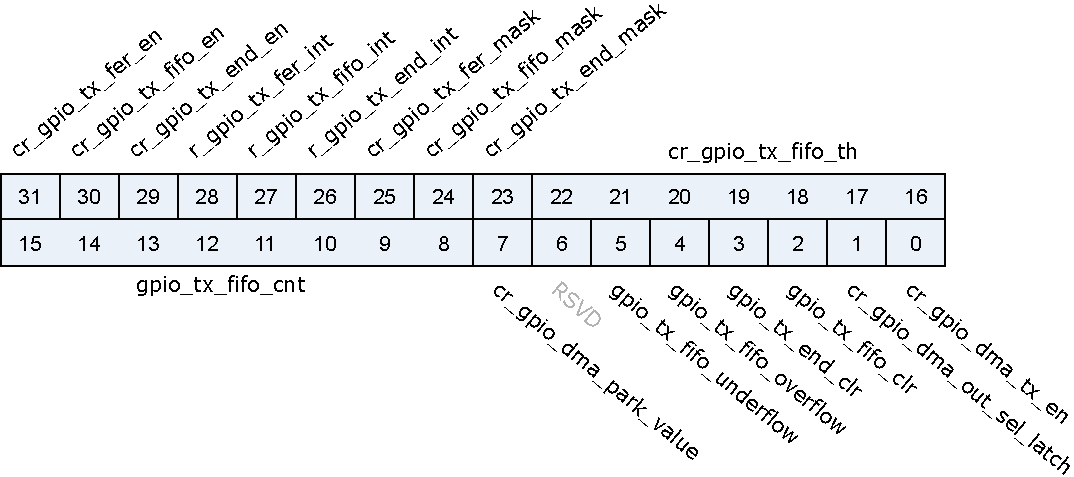
\includegraphics{glb_gpio_cfg143.pdf}
\end{figure}

\regdes{31&cr\_gpio\_tx\_fer\_en&r/w&1'b1&Interrupt enable of gpio\_tx\_fer\_int (GPIO DMA FIFO Underflow or Overflow)\\\hline
30&cr\_gpio\_tx\_fifo\_en&r/w&1'b1&Interrupt enable of gpio\_tx\_fifo\_int \\\hline
29&cr\_gpio\_tx\_end\_en&r/w&1'b1&Interrupt enable of gpio\_tx\_end\_int\\\hline
28&r\_gpio\_tx\_fer\_int&r&1'b0&GPIO TX FIFO error interrupt, auto-cleared when FIFO overflow/underflow error flag is cleared\\\hline
27&r\_gpio\_tx\_fifo\_int&r&1'b0&GPIO TX FIFO ready (tx\_fifo\_cnt > tx\_fifo\_th) interrupt, auto-cleared when data is pushed\\\hline
26&r\_gpio\_tx\_end\_int&r&1'b0&GPIO TX END Interrupt (GPIO DMA FIFO Empty)\\\hline
25&cr\_gpio\_tx\_fer\_mask&r/w&1'b1&Interrupt mask of gpio\_tx\_fer\_int\\\hline
24&cr\_gpio\_tx\_fifo\_mask&r/w&1'b1&Interrupt mask of gpio\_tx\_fifo\_int\\\hline
23&cr\_gpio\_tx\_end\_mask&r/w&1'b1&Interrupt mask of gpio\_tx\_end\_int\\\hline
22:16&cr\_gpio\_tx\_fifo\_th&r/w&7'd0&TX FIFO threshold, dma\_tx\_req will not be asserted if tx\_fifo\_cnt is less than this value\\\hline
15:8&gpio\_tx\_fifo\_cnt&r&8'd128&TX FIFO available count\\\hline
7&cr\_gpio\_dma\_park\_value&r/w&1'b0&1: park at high level when TX FIFO empty \par 0: park at low level when TX FIFO empty
\\\hline
6&RSVD& & & \\\hline
5&gpio\_tx\_fifo\_underflow&r&1'b0&Underflow flag of TX FIFO, can be cleared by tx\_fifo\_clr\\\hline
4&gpio\_tx\_fifo\_overflow&r&1'b0&Overflow flag of TX FIFO, can be cleared by tx\_fifo\_clr\\\hline
3&gpio\_tx\_end\_clr&w1c&1'b0&Interrupt clear of gpio\_tx\_end\_int\\\hline
2&gpio\_tx\_fifo\_clr&w1c&1'b0&Clear signal of TX FIFO\\\hline
1&cr\_gpio\_dma\_out\_sel\_latch&r/w&1'b0&1 : select latch format (8bit set/8bit clr) , 0 : select 16bit output value\\\hline
0&cr\_gpio\_dma\_tx\_en&r/w&1'b0&Enable signal of dma\_tx\_req/ack interface\\\hline

}
\subsection{gpio\_cfg144}
\label{glb-gpio-cfg144}
地址:0x20000b04
 \begin{figure}[H]
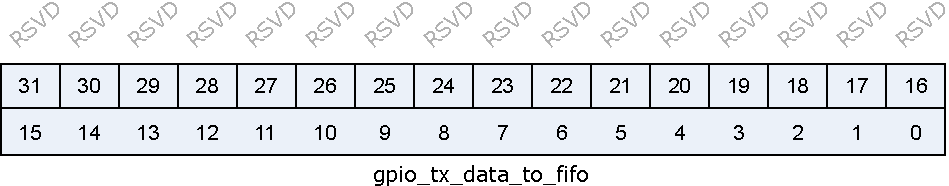
\includegraphics{glb_gpio_cfg144.pdf}
\end{figure}

\regdes{31:16&RSVD& & & \\\hline
15:0&gpio\_tx\_data\_to\_fifo&w&x&\\\hline

}
